\documentclass[output=paper]{langscibook}
\author{Ida Larsson\orcid{}\affiliation{Østfold University College, Halden} and Björn Lundquist\affiliation{The Arctic University of Norway, Tromsø}}
\title{The development of Swedish particle placement}
\abstract{This paper is concerned with the word order of particle constructions in the history of Swedish. Unlike the other Germanic languages, present-day Swedish only allows the order particle–object. In older Swedish, both of the orders particle–object and object–particle were possible, as in e.g. present-day Norwegian. We trace the development of the present-day Swedish word order in texts from the 15\textsuperscript{th} to the 19\textsuperscript{th} centuries. Furthermore, we show that the development is not tied to changes in pronominal object shift, and suggest that the present-day word order is a consequence of a reanalysis of the particle from phrasal modifier to head (cf. the Head Preference Principle proposed by \citealt{van_Gelderen2004}).

\keywords{argument placement, Head Preference Principle, Late Modern Swedish, pronominal object shift, verb particle}
}
\IfFileExists{../localcommands.tex}{
  \addbibresource{../localbibliography.bib}
  % add all extra packages you need to load to this file

\usepackage{tabularx,multicol}
\usepackage{url}
\urlstyle{same}

\usepackage{listings}
\lstset{basicstyle=\ttfamily,tabsize=2,breaklines=true}

\usepackage{langsci-basic}
\usepackage{langsci-optional}
\usepackage{langsci-lgr}
\usepackage{langsci-gb4e}

\usepackage{todonotes}

\usepackage[linguistics]{forest}
\usepackage{soul}
\usepackage{subfigure}
\usepackage{longtable}
\usepackage{enumitem}

  \newcommand*{\orcid}{}
%\newcommand{\keywords}[1]{\textbf{#1}}


\makeatletter
\let\theauthor\@author
\makeatother

\newcommand{\keywords}[1]{\textbf{Keywords:} #1}


\DeclareNewSectionCommand
  [
    counterwithin = chapter,
    afterskip = 2.3ex plus .2ex,
    beforeskip = -3.5ex plus -1ex minus -.2ex,
    indent = 0pt,
    font = \usekomafont{section},
    level = 1,
    tocindent = 1.5em,
    toclevel = 1,
    tocnumwidth = 2.3em,
    tocstyle = section,
    style = section
  ]
  {appendixsection}

\renewcommand*\theappendixsection{\Alph{appendixsection}}
\renewcommand*{\appendixsectionformat}{\appendixname~\theappendixsection\autodot\enskip}
\renewcommand*{\appendixsectionmarkformat}{\appendixname~\theappendixsection\autodot\enskip}
 
  %% hyphenation points for line breaks
%% Normally, automatic hyphenation in LaTeX is very good
%% If a word is mis-hyphenated, add it to this file
%%
%% add information to TeX file before \begin{document} with:
%% %% hyphenation points for line breaks
%% Normally, automatic hyphenation in LaTeX is very good
%% If a word is mis-hyphenated, add it to this file
%%
%% add information to TeX file before \begin{document} with:
%% %% hyphenation points for line breaks
%% Normally, automatic hyphenation in LaTeX is very good
%% If a word is mis-hyphenated, add it to this file
%%
%% add information to TeX file before \begin{document} with:
%% \include{localhyphenation}
\hyphenation{
anaph-o-ra
Dor-drecht
mono-mor-phe-mic
Swed-ish
sche-mat-ic
Viska-da-li-an
An-ders-son
dia-lekt-forsk-ning
dra-ma-språk
bref-vex-ling
Ak-tu-ell
folk-livs-forsk-ning
Þor-björg
Ak-ti-ons-art
Upp-sala
myck-en
}

\hyphenation{
anaph-o-ra
Dor-drecht
mono-mor-phe-mic
Swed-ish
sche-mat-ic
Viska-da-li-an
An-ders-son
dia-lekt-forsk-ning
dra-ma-språk
bref-vex-ling
Ak-tu-ell
folk-livs-forsk-ning
Þor-björg
Ak-ti-ons-art
Upp-sala
myck-en
}

\hyphenation{
anaph-o-ra
Dor-drecht
mono-mor-phe-mic
Swed-ish
sche-mat-ic
Viska-da-li-an
An-ders-son
dia-lekt-forsk-ning
dra-ma-språk
bref-vex-ling
Ak-tu-ell
folk-livs-forsk-ning
Þor-björg
Ak-ti-ons-art
Upp-sala
myck-en
}
 
  \togglepaper[1]%%chapternumber
}{}

% todo
% bibs
% jambox
% *
% alignment brackets
\begin{document}
\maketitle 

\section{Introduction}\label{sec:lalu:1}

\begin{sloppypar}
As is well known, standard present-day Swedish differs from all of the other (North) Germanic languages in only allowing the order verb particle–object, cf. \REF{ex:lalu:1a} and \REF{ex:lalu:1b} (see e.g. \citealt{Svenonius1996, Svenonius2003, Svenonius1996}; \citealt{Toivonen2003}; \citealt{Lundquist2014Active}).\footnote{Unless otherwise indicated, all examples are from present-day Swedish.}
\end{sloppypar}

\ea\label{ex:lalu:1}
\ea[]{\label{ex:lalu:1a}
\gll  Han   kastade   bort     boken/den.\\
      he           threw     away  book\textsc{.def}/it\\}
\ex[*]{ \label{ex:lalu:1b}
\gll   Han  kastade   boken/den   bort. \\
        he      threw     book\textsc{.def}/it    away\\
\glt       ‘He threw the book away.'}
\z
\z


This restricted word order is a rather recent development in the history of Swedish. Up until the 18\textsuperscript{th} century, Swedish showed variation in word order in a way that greatly resembles modern Norwegian dialects and Icelandic (as well as English): pronouns tended to precede particles \REF{ex:lalu:2a}, whereas full DP objects often (but not always) followed the particle (\ref{ex:lalu:2}b–c; see \citealt{LarssonLundquist2014}).


\ea\label{ex:lalu:2}
\ea\label{ex:lalu:2a}
\gll  slogo  resan       mik     {i häll}\\
 beat     giant.\textsc{def}   me     \textsc{part}\\
  \glt `the giant killed me’ (\textit{Didrik}, ca. 1450, p. 58)

\ex   \label{ex:lalu:2b}
\gll han …   slog  sunder   dørrernæ\\
      he  ~           broke  \textsc{part}       door\textsc{.def.pl}\\
  \glt   ‘he broke the doors’ (\textit{Didrik}, ca. 1450, p. 58)

\ex
\gll oc    slog     swerdit     sunder\\
      and  broke   sword\textsc{.def}   \textsc{part}\\
  \glt  ‘and broke the sword’ (\textit{Didrik}, ca. 1450, p. 48)

\z
\z

This paper is concerned with the development of the strict order particle–object in the history of Swedish. The article has two objectives. First, we aim to give an accurate description of the change in word order with respect to verb particles and direct objects. The focus is on the 17\textsuperscript{th}--19\textsuperscript{th} centuries, which is the period where we see the most rapid change. Secondly, we discuss different ways of modelling the change in a generative framework. We show that the change in particle constructions cannot be a direct consequence of the shift from OV order to VO order in the history of Swedish. We argue that it should not be analyzed in terms of a change in headedness or in available argument positions in the verb phrase, nor can we link it to a general change in pronominal object shift. Instead, we propose that the change is best described as a reanalysis of the particle. We propose that in older Swedish, the particle is a phrasal modifier of a result-encoding phrase, whereas in present-day Swedish it is the head of the said phrase. The change can thus be captured by the so-called Head Preference Principle (\citealt{van_Gelderen2004}). We will see that not all particle-like elements behave in the same way in older Swedish, and that not all elements or contexts change at the same time. Most evidently, in the context of a PP, directional adverbs do not behave like particles in older Swedish, but in present-day Swedish they do. Overall, the category of particles appears to be syntactically more homogeneous in present-day Swedish than in Swedish before the middle of the 17\textsuperscript{th} century. 



The structure of the article is as follows. In \sectref{sec:lalu:2}, we give a brief description of the category of verb particle, in the sense it is used in the literature on the Germanic languages. We also go through the characteristics of particles in present-day Swedish and give an overview of what is included in our study of older Swedish. \sectref{sec:lalu:3} introduces the historical corpus, and in Sections 4 and 5 we present the results from the corpus study. In \sectref{sec:lalu:6}, we discuss possible analyses of the change. We discuss the connection between the change in word order in particle constructions and the shift from OV order to VO order, and possible changes in object shift and VP-internal argument positions, but propose that the change is best understood as a change in the properties of the particle. \sectref{sec:lalu:7} briefly discusses some recent developments and concludes the paper.


\section{Verb particles in Germanic and Swedish}\label{sec:lalu:2}


Verb particles in the Germanic languages in general, and the Nordic languages in particular, have been extensively discussed (see e.g. \citealt{Afarli1985}; \citealt{Den_dikken1995}; \citealt{Svenonius1996}; \citealt{Wurmbrand2000}; \citealt{Dehe2002}; \citealt{RamchandSvenonius2002}; \citealt{Toivonen2003}; \citealt{Aa2015}). Verb particles may at first appear to be a fairly heterogeneous category, but they share some characteristics throughout the Germanic languages, which we discuss below. 



In \sectref{sec:lalu:2.1}, we give a very brief overview of the most characteristic properties of particles. \sectref{sec:lalu:2.2} introduces some standard diagnostics for identifying particles in present-day Swedish. In \sectref{sec:lalu:2.3}, we discuss how particles can be identified in the historical records and look at some problematic cases.


\subsection{Particles}\label{sec:lalu:2.1}

\begin{sloppypar}
Particles have been described as “intransitive prepositions” (e.g. \citealt{Emonds1976}; \citealt{Svenonius1996}; \citealt{Faarlund2019}: 137), where the internal argument has been dropped. The core function of regular prepositions is to locate an external “figure” argument, either spatially or temporally, in relation to an internal “ground” argument; see the locative preposition \textit{i} ‘in’ \REF{ex:lalu:3a}. In the most straightforward instances, particles fulfil a similar function to that of prepositions: they locate a figure argument with respect to an implicit ground; see the adverbial particle \textit{in} ‘in’ in \REF{ex:lalu:3b}. The implicit ground argument of a particle can be realized as a prepositional phrase; see \REF{ex:lalu:3c} where both a particle and a ground-introducing preposition are present.
\end{sloppypar}

\ea\label{ex:lalu:3}
\ea\label{ex:lalu:3a}
\gll  Hon   ställde   mjölken     i     kylskåpet.\\
    she       put     milk\textsc{.def}   in   refridgerator.\textsc{def}\\
\glt `She put the milk in the refrigerator.'

\ex\label{ex:lalu:3b}
\gll  Hon   ställde   in  mjölken.\\
  she   put     in   milk.\textsc{def} \\
  \glt `She put the milk in (the refridgerator).’

\ex\label{ex:lalu:3c}
\gll  Hon   ställde   in   mjölken     i     kylskåpet.\\
  she   put     in   milk.\textsc{def}     in     refrigerator.\textsc{def}\\
\glt    ‘She put the milk in the refrigerator.’

\z
\z


In the examples above, \textit{mjölken} ‘the milk’ is the figure argument, which is located with respect to the ground argument \textit{kylskåpet} ‘the refrigerator’. In \REF{ex:lalu:3b}, the ground is only implicit: the milk is located inside something, and from world knowledge (and context) we can speculate that the ground is most likely a refrigerator.



It is, however, clear that not all verb particles establish a simple figure–ground relation. In example \REF{ex:lalu:4} below, the same verb and particle as in \REF{ex:lalu:3} are used, but the semantic relation is not a simple figure--(implicit) ground relation:


\ea\label{ex:lalu:4}
\gll  Hon   ställde   in   konserten.\\
  she       put         in   concert.\textsc{def}\\
\glt `She cancelled the concert.'

\z

Another characteristic of particles is that they add an endpoint to otherwise atelic event descriptions, as shown in the pair below:


\ea\label{ex:lalu:5}
\ea{
\gll  Han  dansade   i   rummet.      \\
      he         danced   in   room.\textsc{def}\\}\jambox*{ (atelic, locative PP)}
\glt `He danced in the room.'

\ex{
\gll Han  dansade   in   i     rummet.    \\
      he       danced     in     in  room.\textsc{def}\\}\jambox*{(telic, particle\,+\,PP)}
\glt `He danced into the room.'

\z
\z

Due to this property, it has been suggested that the verb particle is associated with a result-encoding phrase inside the verb phrase, which it either heads or modifies (e.g. \citealt{RamchandSvenonius2002}). Support for this idea comes from pairs such as (\ref{ex:lalu:6}a–b) below, where it looks like the particle not only adds an endpoint to a complex event, but also introduces its own argument, similar to a verb:


\ea\label{ex:lalu:6}
\ea[]{
\gll  Han   dansade     sönder   sina        skor     på   fem     minuter.\\
      he       danced     broken   \textsc{poss.refl} shoes   in     five   minutes\\
\glt `He danced his shoes broken in five minutes.'
}
\ex[*]{
\gll Han  dansade   sina        skor     i/på     fem     minuter.\\
        he     danced     \textsc{poss.refl}   shoes     for/in   five   minutes.’\\
\glt `He danced his shoes broken for/in five minutes.'
}
\z
\z

Despite the facts in (\ref{ex:lalu:5}--\ref{ex:lalu:6}), most particles change neither the Aktionsart/telicity nor the valency of the predicate, as already illustrated in \REF{ex:lalu:3} above. That is, particles often modify or specify a result of an event already named by the verb (see \ref{ex:lalu:7}), sometimes in combination with a PP (cf. \ref{ex:lalu:3c}).


\ea\label{ex:lalu:7}
\gll  Han     stängde   (igen)   fönstret.\\
he       closed     \textsc{part}     window.\textsc{def}\\
\glt `He closed the window.'
\z

From a morphosyntactic perspective, it is important to point out that even in clearly non-transparent verb-particle combinations, the verb and the particle do not form a syntactic word. This is most evident from the Germanic V2 languages, where the syntactic subject and sentence adverbs may intervene between verb and particle when the main verb moves to the V2 position (see \citealt{Afarli1985}):


\ea\label{ex:lalu:8}
\gll  Därför   ställde   hon     inte     in   konserten.\\
therefore  put   she   not     in     concert.\textsc{def}\\
\glt `Therefore, she didn’t cancel the concert.'
\z


We will return to the formal analysis of particles in \sectref{sec:lalu:6} below. For now, the reader should keep in mind the following properties of verb particles: they behave like intransitive prepositions, they tend to induce or modify endpoints in event descriptions, and they behave like independent words. In the next section we will look at diagnostics for particles in present-day Swedish.


\subsection{Identifying particles in present-day Swedish}\label{sec:lalu:2.2}

It is often not evident how verb particles should be identified in corpora (see e.g. \citealt{LarssonRoxendal2020} for discussion). Words from different classes (e.g. prepositions, adverbs, and adjectives) can be used as particles. Only in a few exceptional cases can particles be lexically identified; in present-day Swedish, this is the case for instance with \textit{ihjäl} ‘to death’ which is only used as a verb particle, or \textit{an} ‘to’ which is always either a particle or a prefix.


\begin{sloppypar}
There are, however, some prosodic and syntactic diagnostics to distinguish particle constructions from constructions with verb\,+\,PP, or verb\,+\,adjectival small clause. In present-day Swedish, word order is often used as a diagnostic: since a particle always precedes the object, examples like those in \REF{ex:lalu:9} must involve AdvPs or APs.
\end{sloppypar}


\ea\label{ex:lalu:9}
\ea
\gll  Hon   körde   honom   hem.  \\
    she     drove   him     home\\
\glt `She drove him home.'

\ex
\gll  Hon   torkade   den   ren.\\
    she     wiped   it     clean\\
\glt `She wiped it clean.'
\z
\z

\begin{sloppypar}
In traditional grammars, prosody is an important way of identifying particles in present-day Swedish (see e.g. \citealt{TelemanEtAl1999}/3: 417). In \REF{ex:lalu:10a}, verb\,+\,particle form a maximal prosodic word (in the sense of \citealt{MyrbergRiad2015}), and the accent is on the particle (as indicated with the capital letters). In \REF{ex:lalu:10b}, the locative preposition forms a (prosodic) constituent with the noun phrase, and the verb is accented.
\end{sloppypar}

\ea\label{ex:lalu:10}
\ea\label{ex:lalu:10a}
\gll  skriva   PÅ   kontraktet\\
    write     \textsc{part}   contract\textsc{.def}\\
\glt `sign the contract'

\ex\label{ex:lalu:10b}
\gll  SKRIVA  på   en  bit     papper \\
    write     on   a   piece    paper\\
\glt `write on a piece of paper'
\z
\z


Moreover, the object and particle do not form a syntactic constituent that can be topicalized. Compare again the particle construction in \REF{ex:lalu:11a} with the locative prepositional phrase in \REF{ex:lalu:11b}.


\ea\label{ex:lalu:11}
\ea[*]{\label{ex:lalu:11a}
\gll  På   kontraktet     skrev   jag.\\
    \textsc{part}     contract\textsc{.def}   wrote   I\\
    Intended: ‘The contract, I signed.'
}
\ex[]{\label{ex:lalu:11b}
\gll  På   en   bit   papper   skrev     jag.\\
    on   a     piece  paper   wrote   I\\
\glt `On a piece of paper, I wrote.’\\
}
\z
\z


On the other hand, it is sometimes possible to topicalize the particle by itself, at least in a limited set of contexts, and with directional particles (see \citealt{TelemanEtAl1999}/3: 427). Typically, contrast is required, as in \REF{ex:lalu:12}. In the same contexts, verbs can be topicalized, stranding the object; see \REF{ex:lalu:13}. Prepositions cannot be topicalized in the same manner.


\ea\label{ex:lalu:12}
\gll  Hon   gav     honom   rejält       med   stryk,     men   ihjäl\\
she     gave     him   properly     with   beating     but     \textsc{part}\\

\gll  slog   hon  honom  inte. \\
beat   she   him     not\\
\glt `She gave him a proper beating, but she didn’t beat him to death.'
\ex\label{ex:lalu:13}
\gll  Kysst     har   jag   henne   inte,   bara   hållit  henne   i     handen.\\
kissed   have   I   her     not     only   held   her   in   hand\textsc{.def}\\
\glt `I haven’t kissed her, only held her hand.' \citep{Holmberg1997}\\
\z


Another way of identifying particles in present-day Swedish is that they obligatorily incorporate into participles (even in verbal passives; see \citealt{Lundquist2014Passives} and references therein). Consider the contrast between the canonical periphrastic passive in \REF{ex:lalu:14a} and the pseudopassive in \REF{ex:lalu:14b}.


\ea\label{ex:lalu:14}
\ea\label{ex:lalu:14a}
\gll  Kontraktet   blev   på-skrivet.\\
    contract\textsc{.def}   was   \textsc{part-}write.\textsc{ptcp}\\
\glt `The contract was signed.'

\ex\label{ex:lalu:14b}
\gll  Kontraktet     har   blivit   skrivet     på. \\
    contract\textsc{.def}   has   been   write.\textsc{ptcp}   on\\
\glt `The contract has been written on.’ (pseudopassive)\\
\z
\z


In \REF{ex:lalu:14a}, \textit{på} is incorporated into the passive participle, and the only interpretation is that the passive involves the particle verb \textit{skriva på} ‘sign’. In \REF{ex:lalu:14b}, on the other hand, \textit{på} has not been incorporated and must therefore be analyzed as a locative preposition. The complement of the preposition has been promoted to subject, stranding the preposition.



Word order, prosody, constituency, and incorporation can thus be used to identify particles in present-day Swedish, at least in many cases. We return to some more problematic cases in the next section, where we discuss how we can identify particles in older Swedish texts. 


\subsection{The particles in this study}\label{sec:lalu:2.3}

None of the diagnostics discussed above can be directly applied to historical corpus data. Rather, to identify particles in older, written texts, we have to rely partly on our intuitions about the properties of the present-day Swedish translational equivalents of the relevant particle-like elements we find in the corpus. In this study, we have included constructions that would have the word order and prosody of present-day Swedish particles. Moreover, we have used the possibility of an object \textit{preceding} a prepositional element to identify particles in older Swedish (as in present-day Icelandic and Norwegian): in older Swedish, the order object–particle is possible, whereas the order complement–preposition is not.\footnote{There is one systematic exception, involving \textit{r}{}-pronouns (e.g. \textit{der} ‘there’), which precede prepositions in Old Swedish \citep{Delsing2014Svenskans}. It is also possible that complex prepositions like \textit{emot} ‘toward’ could follow their complements in older Swedish (Falk p.c.) – this would make it particularly difficult to distinguish prepositional from particle uses.}  Examples with the order object–preposition/particle are therefore included among the particle constructions in the historical study.\footnote{In
    15th–18th century Swedish, the preposition \textit{till} ‘to’ can follow a benefactive object. Examples like (i) are included among the particle constructions.

    \ea
    \gll skrev   och   Påwen   till\\
    wrote   also  pope.\textsc{def}   to\\
    \glt ‘wrote also to the pope’ (Swart, 1560, p. 52)
    \z

    In present-day Swedish, the only possible order is \textit{till}\,+\,DP, and \textit{till} heads a PP with the benefactive/goal as a complement. That is, the modern correspondent to (i) is not included among the particle constructions. In the historical study, only examples with the order DP–\textit{till} have been included, and, given that there is word order variation in particle constructions, this might skew the quantitative data somewhat in favour of the older word order.
}



However, even in present-day Swedish, there are cases where the diagnostics mentioned do not disambiguate particles from prepositions or adverbs. We will look at some core cases below and specify how we treat them in the diachronic corpus.

\subsubsection{Directional prepositions} 

As pointed out by \citet{Svenonius2003}, directional prepositions are accented in Swedish, and therefore prosodically indistinguishable from particles. In traditional grammars, examples like \REF{ex:lalu:15a}, with stress on the preposition \textit{i} ‘in’, are treated as particle constructions, due to their prosody, whereas the locative example in \REF{ex:lalu:15b}, with stress on the verb, is not.


\ea\label{ex:lalu:15}
\ea\label{ex:lalu:15a}
\gll  Hon   hoppade    i   vattnet. \\
    she     jumped     in   water\textsc{.def}\\
\glt `She jumped into the water.'

\ex\label{ex:lalu:15b}
\gll  Hon   HOPPADE   i   vattnet. \\
    she     jumped       in   water\textsc{.def}\\
\glt `She jumped in the water.'
\z
\z


It is generally difficult to test whether the preposition/particle in examples like \REF{ex:lalu:15a} incorporates into a participle, since there are other interfering restrictions on periphrastic passives in Swedish (see e.g. \citealt{Engdahl2006}). Some constituency tests fail with directional prepositions; \REF{ex:lalu:16a} can for instance only have a locative reading. However, examples like \REF{ex:lalu:16b}, which are directional as well, and have stress on \textit{över}, suggest that the preposition and DP might form a constituent (see \citealt{Tungseth2006}). In other words, \REF{ex:lalu:16a} shows that directional prepositions can behave like particles (see \ref{ex:lalu:11a} above), but \REF{ex:lalu:16b} shows that they do not necessarily do so.


\ea\label{ex:lalu:16}
\ea\label{ex:lalu:16a}
\gll  I     vattnet   hoppade   hon. \\
    in     water\textsc{.def}  jumped   she\\
\glt `She jumped in the water\textsc{’}\\
    NOT: ‘She jumped into the water.'

\ex\label{ex:lalu:16b}
\gll  Det  var   över   gatan     hon   gick.\\
    it     was  over   street\textsc{.def}   she   went\\
\glt `It was across the street she went.'     (\citealt{Svenonius2003}: 12b)\\
\z
\z


As discussed in \sectref{sec:lalu:2} above, many prepositional particles can be said to take an object that has the thematic role of figure, whereas the ground argument of PPs remains implicit. In directional constructions like \REF{ex:lalu:16a}, the subject is, however, the figure, and the DP \textit{vattnet} ‘the water’ is the ground.



In the present study, we have followed traditional grammars and also included cases with prepositional elements that take ground arguments among the particles, if other diagnostics (e.g. prosody) point toward a particle analysis. In this way, we can investigate whether these constructions pattern with other particles in the history of Swedish. We will, however, code them as “ground” particles and take their special semantics into consideration in the analysis.



\subsubsection{Directional adverbs preceding directional prepositions} 
Another difficulty involves directional particles/adverbs in the context of a PP, as in \REF{ex:lalu:17a}. Here, it is possible to treat the adverb as part of the PP, and that is what is also suggested by the possibility of the word order in the authentic example in \REF{ex:lalu:17b} and the topicalization in \REF{ex:lalu:17c}.


\ea\label{ex:lalu:17}
\ea\label{ex:lalu:17a}
\gll  Hon   kastade   upp    honom   i   luften.\\
    she     threw   up   him     in     air\textsc{.def}\\
\glt `She threw him up in the air.’\\

\ex\label{ex:lalu:17b}
\gll  Hon   kastade   honom   upp   i   luften.\\
    she     threw   him     up   in   air\textsc{.def}\\
\glt `She threw him up in the air.’ (Lindgren, \textit{Känner du Pippi Långstrump}, 1947)\\
\ex\label{ex:lalu:17c}
\gll Upp   i   luften   kastade   hon   honom. \\
    up     in   air.\textsc{def}   threw   she   him\\
\glt `She threw him up in the air.’     (from \citealt{LarssonLundquist2014})\\
\z
\z


The examples in \REF{ex:lalu:17} do not necessarily all have the same structure. In present-day Swedish, \REF{ex:lalu:17a} requires an analysis of \textit{upp} as a particle, whereas in \REF{ex:lalu:17b} the word order (object–adverb) rules out that analysis. In older Swedish, on the other hand, \REF{ex:lalu:17b} could also be analyzed as involving a particle. We have therefore included both cases corresponding to \REF{ex:lalu:17a} and \REF{ex:lalu:17b} in the study, but we have annotated them so that they can easily be treated separately. As we will see in the following, the word order in \REF{ex:lalu:17b}, with the object preceding the particle in the context of a PP, is the rule in older Swedish, but gradually becomes less frequent.



\subsubsection{Modified particles} 
We have excluded a few cases with modified particles, like \REF{ex:lalu:18}. Here, the particle necessarily follows the object, in (older) Swedish as in the other Germanic languages (but see \sectref{sec:lalu:7} below). Examples like these are rare in the historical texts, and they are uncommon even in the present-day corpora; we return to them briefly in \sectref{sec:lalu:7}. Modified particles are not included in the corpus study.


\ea\label{ex:lalu:18}
\gll Vi    kastade   \{stenen\}     långt  ut \{*stenen\}.\\
we    threw       rock\textsc{.def}   far   out     rock\textsc{.def}    \\
\glt `We threw the rock far out.'
\z


\subsubsection{Particles and reflexive objects} 
Simple reflexive objects show a somewhat variable behaviour with respect to particle placement in present-day Swedish. We find at least three patterns, as exemplified in \REF{ex:lalu:19} below (see \citealt{Lundquist2014Reflexive} and references therein).


\ea\label{ex:lalu:19}
\ea\label{ex:lalu:19a}
\gll  Hon   tog     sig     in   i     rummet.\\
    she       took   \textsc{refl}   in   in     room\textsc{.def}\\
\glt `She got herself into the room.’\\

\ex\label{ex:lalu:19b}
\gll  Hon   la     sig ner     i   sängen.\\
    she     lay   \textsc{refl}   down   in   bed.\textsc{def}\\
  \glt `She lay down in the bed.’ \\
\ex\label{ex:lalu:19c}
\gll Hon   klädde   upp   sig   igår. \\
    she     dressed   up   \textsc{refl}   yesterday\\
\glt `She dressed up yesterday.’\\
\z
\z


In \REF{ex:lalu:19a}, the reflexive object precedes the particle, and the particle carries typical particle stress. In \REF{ex:lalu:19b}, the reflexive also precedes the particle, but the particle does not carry particle stress – the stress is on the verb. Finally, \REF{ex:lalu:19c} has the typical word order of a present-day Swedish particle construction, with the particle preceding the reflexive. We will exclude reflexives from our statistical analysis of the change, but we will briefly comment on the first attestations of the order in \REF{ex:lalu:19c}. It should be noted that this word order is absent in the other North Germanic languages.



\subsubsection{Particles that describe co-movement of subject and object} 
In the present study, we have also disregarded cases where the particle gives the direction of both the subject and the object argument (see \citealt{Toivonen2003}). An example is given in \REF{ex:lalu:20}; here both \textit{I} and \textit{she} go out.


\ea\label{ex:lalu:20}
\gll  Jag     följde     henne   ut.\\
I         followed   her     out\\
\glt `I followed her out.'
\z


In these cases, objects have to precede particles in present-day Swedish. The particle does not carry particle stress, and it cannot be incorporated into passives.



Finally, we have excluded particle verbs with clausal complements, as clausal complements always followed particles in older Swedish, as they do in the other North Germanic languages and English (e.g., \textit{I found out that John won the race/*I found that John had won the race out}.)



To summarize, we have largely followed traditional Swedish grammars when identifying particles in older Swedish texts. We have intentionally been rather liberal and included everything that would lend itself to a particle analysis in present-day Swedish, since this makes it possible for us to investigate how the particle category should be delimited, rather than assuming an \textit{a priori} stable category. However, we do not include constructions with reflexive or clausal objects, nor examples where the particle follows the object in present-day Swedish. In addition to present-day Swedish particles, we have included cases that behave like particle constructions in older Swedish (e.g., by allowing word order variation). This includes cases where present-day Swedish has a prefixed verb, e.g., older Swedish \textit{billa någon in} for present-day \textit{inbilla någon} ‘make somebody believe’, or older \textit{gå någon an} for present-day \textit{angå någon} ‘concern somebody’.


\section{The corpus}\label{sec:lalu:3}


The study uses a corpus of 18 texts from the period ca. 1450–1849. Together with data from previous studies, one text (\textit{Didrik av Bern}, ca. 1450) represents Late Old Swedish. The choice of this particular text is based on the results from \citet{Ljunggren1932}, who shows that it has a considerable number of particles that follow the non-finite verb; this allows us to investigate the order between particle and object (independently of OV order). In addition, the corpus includes several texts that are generally assumed to reflect the language of Central Sweden (Stockholm, Uppsala, and surroundings) better than other texts from the same period, for instance \textit{Peder Swarts krönika} (1560), and the autobiography of Agneta Horn (1657). Kiöping’s travel description (published in 1674) and the edition by Salvius (1743) are versions of the same text, and therefore allow for good comparison. Finally, the corpus contains 13 plays from the period 1734 to 1849, taken from the corpus of Swedish drama dialogue \citealt{MarttalaStromquist2001}). As historical sources, these plays are particularly interesting and useful, since the authors often attempt to reflect the spoken language of their time. As we will see in \sectref{sec:lalu:5}, the plays can, however, be more or less liberal.



In the following, we will refer to the texts with reference to the author’s year of birth (when known), rather than the dating of the text; since our interest is in the grammatical competence of the individual, we assume that year of birth is more important than the time of writing or publication. The first text in our corpus that belongs to the traditional Late Modern Swedish period is the play \textit{Svenska sprätthöken} by Carl Gyllenborg (born 1679). 



In all, the data consists of 1525 sentences with particles that have been manually excerpted and annotated. In the presentation below, we restrict the discussion to sentences with pronominal or full DP objects, and further exclude reflexive objects and double object constructions; double objects will however be discussed briefly in \sectref{sec:lalu:6} below. The quantified data includes 1144 sentences with verb particles. These have been annotated for word order (object–particle or particle–object) and type of object (pronoun – full DP). In addition, we have distinguished between different types of particles: prepositions (e.g., \textit{i} ‘in’), adverbs (\textit{ut} ‘out’), complex particles (\textit{uti} ‘in’, \textit{emot} ‘toward’), and elements like \textit{ihjäl} ‘to death’, which always have a particle function. We also note the presence of a prepositional phrase related to the particle (as in \textit{throw up in the air}). We have further annotated what meaning the particle carries (directional, metaphorical etc.), but since it is often hard to come up with strict criteria for different types of meaning, we will only briefly make reference to this level of annotation.



In \sectref{sec:lalu:4}, we describe the word order in particle constructions in Old and Early Modern Swedish up until the beginning of the 17\textsuperscript{th} century. In \sectref{sec:lalu:5}, we look more closely at the period from the middle of the 17\textsuperscript{th} century onwards, which is when the modern word order was established.


\section{Particle placement in Old and Early Modern Swedish}\label{sec:lalu:4}


Old Swedish had the same word order possibilities in particle constructions as the other North Germanic languages did (see e.g. \citealt{Ljunggren1932}; \citealt{Diderichsen1941}; \citealt{Hroarsdottir2008}). There was considerable variation in word order, not least since the languages alternated between OV and VO structures. In \sectref{sec:lalu:4.1}, we briefly describe the word order possibilities in Early Old Swedish (with data from previous work). \sectref{sec:lalu:4.2} is concerned with the patterns we find in texts from the Late Old Swedish period to the beginning of the 17\textsuperscript{th} century, where VO order was increasingly becoming the norm.


\subsection{Particle placement in Early Old Swedish}\label{sec:lalu:4.1}

The Old North Germanic languages all showed variation between VO and OV order.\footnote{According to \citet{Delsing1999}, there was a drop in the frequency of OV in the 14\textsuperscript{th} century. OV was, however, to some extent revived again towards the end of the 15\textsuperscript{th} century, and it survived (to some degree) until the 18\textsuperscript{th} century (see also \citealt{Petzell2011}). See \sectref{sec:lalu:6} for further discussion.} Particles and objects could therefore either follow or precede a non-finite verb, and the order between particle and object could also vary. In the Old Swedish medieval laws, it is common for both object and particle to precede a non-finite verb, as in \REF{ex:lalu:21a} (examples from \citealt{Ljunggren1932} and Falk p.c.).\footnote{All Early Old Swedish examples have been checked with the electronic text versions available through \textit{Fornsvenska textbanken}, which is available here: \url{https://project2.sol.lu.se/fornsvenska/}}  We also find the VO patterns of present-day Norwegian and Icelandic; see \REF{ex:lalu:21b} where the object precedes the particle, and \REF{ex:lalu:21c} where the particle precedes the object. As far as we are aware, the order particle–object–verb is not attested (cf. \citealt{Hroarsdottir2008} on Icelandic).


\ea\label{ex:lalu:21}
\ea\label{ex:lalu:21a} O–part–V:  \\
\gll  vil     maþer   træþi       up   taka \\
    want     man     plowing    up   take\textsc{.inf} \\
\glt `someone wants to start plowing’ (EWL, 13\textsuperscript{th} c.)\\

\ex\label{ex:lalu:21b} V–O–part:     \\
\gll  þa     skal     han   bindæ   han   wiþ \\
    then   should   he   tie\textsc{.inf}   him   \textsc{part} \\
\glt `then should he tie him to the crime’ (UL, 13\textsuperscript{th} c.)\\

\ex\label{ex:lalu:21c}  V-part–O:     \\
\gll  Vil     by   takæ       in   mark   sinæ \\
    want  farm   fence.\textsc{inf}   in   land   \textsc{poss.refl} \\
\glt `a farm wants to fence in its land’ (EWL, 13\textsuperscript{th} c.)\\
\z
\z

The general rule is that object and particle appear on the same side of the verb, but there are also examples where the object and the particle appear on opposite sides of the verb; see \REF{ex:lalu:22}. These cases appear to be less common (see \citealt{Ljunggren1932}), and it is hardly a coincidence that \REF{ex:lalu:22b} involves a heavy object.


\ea\label{ex:lalu:22}
\ea\label{ex:lalu:22a} O--V–part:  \\
\gll þa     skal   lanz       asyn       næmnæ       til\\
    then   shall   land.\textsc{gen}   inspection   appoint.\textsc{inf}   \textsc{part} \\
\glt `then shall an inspection of the land be appointed’ (EWL, 13\textsuperscript{th} c.; from Falk p.c.)\\

\ex \label{ex:lalu:22b}part–V–O:     \\
\gll þa     skal   af  takæ.   hemfylgh   sinæ       alt   þét \\
    then   shall   away  take.\textsc{inf}  dowry     \textsc{poss.refl}   all   that \\

\gll ær       vnöt         ær...\\
    which   unnecessary   is \\
\glt `shall then take away all the dowry that is necessary’ (EWL, 13\textsuperscript{th} c.; from \citealt{Ljunggren1932})\\
\z
\z



In the oldest texts, particles precede the non-finite verb in a majority of the cases: 75\% in the Elder Westrogothic Law (EWL, ca. 1220) and 87\% in the Law of Uppland (UL, 1296) according to \citet[95]{Ljunggren1932}. This is not unexpected, given that OV order dominates in these laws. In later texts, with more VO order, particles more often follow the verb. In Early Old Swedish, particles do not precede finite verbs in V2 position (with a small number of exceptions), but this becomes a possibility from the 14\textsuperscript{th} century onwards. 



However, particle placement does not fully pattern with other OV and VO structures (as they seem to in the shift from OV to VO in Icelandic; see \citealt{Hroarsdottir2008}). Instead, the order exemplified in \REF{ex:lalu:22b}, with the particle preceding the non-finite verb and the object after the verb, becomes more common when OV order is lost, presumably due to the emerging possibility of incorporating the particle into the verb. As shown by \citet{Ljunggren1932,Ljunggren1937}, the incorporation of particles into verbs started to be frequent in the 15\textsuperscript{th} century (particularly in formal genres, influenced by Latin).



In the next section, we look more closely at particle placement in three texts from the period 1450–1674.


\subsection{A closer look at the ordering of post-verbal objects and particles}\label{sec:lalu:4.2}

In this section, we investigate the three oldest texts in the corpus, namely \textit{Didrik av Bern} (\textit{Didrik}, ca. 1450), \textit{Peder Swarts krönika} (Swart, 1560), and \textit{Nils Matson Kiöpings resa} (Kiöping, 1674). Although they were written in different centuries, they largely show the same patterns with respect to the ordering of objects and particles, at least once we disregard OV patterns and particle incorporation. 



Firstly, there is a clear difference between pronominal and non-pronominal objects in all three texts; see \tabref{tab:lalu:1}. Overall, around half of the non-pronominal objects follow particles in the texts, whereas only 8\% of the pronouns do.


\begin{table}
\caption{The placement of post-verbal particles and objects in three older Swedish texts.}
\label{tab:lalu:1}
\begin{tabularx}{.9\textwidth}{lXXX}
\lsptoprule
Text & Part--pronoun & Part–DP & Total\\
\midrule
\textit{Didrik} (ca. 1450) & 2/18 (11\%) & 41/97 (42\%) & 43/115 (37\%)\\
Swart (1560) & 3/26 (12\%) & 35/74 (47\%) & 38/100 (38\%)\\
Kiöping (1674) & 1/27 (4\%) & 30/49 (61\%) & 31/76 (41\%)\\
\midrule
TOTAL & 6/71 (8\%) & 106/220 (48\%) & 112/291 (38\%)\\
\lspbottomrule
\end{tabularx}
\end{table}

Both indefinite and definite full DPs can precede particles in all three texts. Examples from \textit{Didrik av Bern} are given in \REF{ex:lalu:23}:


\ea\label{ex:lalu:23}
\ea
\gll  oc     brøt   mang   slot       nid\\
    and     tore   many   castles   down \\
\glt `and tore down many castles’ (\textit{Didrik}, ca. 1450, p. 32)\\

\ex
\gll  slog     swerdit     sunder \\
    broke   sword\textsc{.def}   \textsc{part}\\
\glt `broke the sword’ (\textit{Didrik}, ca. 1450, p. 48)\\
\z
\z


Heavy DPs are, on the other hand, placed after the particle, as in \REF{ex:lalu:24}:


\ea\label{ex:lalu:24}
\gll  Sände   så  in   till   Stocholm     en   gammall   Biscop,   benempd…\\
sent       so    in   to     Stockholm     an   old       Bishop   called\\
\glt `then sent into Stockholm an old Bishop, called…’ (Swart 1560: 4)\\
\z


As we saw in \sectref{sec:lalu:2} above, it is not always clear whether an adverb should be treated as a particle in the context of a directional PP. The order adverb–object–PP forces a particle analysis (given standard assumptions), but in the three older Swedish texts, there are no such examples. Rather, in the context of a PP, the object always precedes the adverb, if it is not extraposed as in \REF{ex:lalu:24}. Examples are given in \REF{ex:lalu:25}; there are in all about 40 such examples in the three texts.


\ea\label{ex:lalu:25}
\ea\label{ex:lalu:25a}
\gll  skött  han   eelden     in     på   Staden\\
    shot     he   fire\textsc{.def}     in   on   town\textsc{.def} \\
\glt `he shot in fire on the town’ (Swart 1560: 30)\\

\ex\label{ex:lalu:25b}
\gll  burit     Wedh   och   Eeld   up   i   Huuset \\
    carried   wood   and   fire   up   to   house\textsc{.def}\\
\glt `carried wood and fire up to the house’ (Kiöping, b. 1621, p. 66)\\
\z
\z


Moreover, different prepositions can show different patterns, and they should probably not all be given the same analysis. For instance, with the particle verb \textit{slå till} ‘strike’, the particle \textit{till} always precedes the object \REF{ex:lalu:26}.\footnote{This pattern is also found in modern Norwegian with \textit{slå til}. \citet{Tungseth2006} suggests that \textit{til} is not a particle, but heads a PP.} Compare this with \textit{slå aff} ‘beat off’ in \REF{ex:lalu:27}, where \textit{aff} follows the object. There are 8 examples with \textit{slå till} ‘strike’ or \textit{ramma till} ‘strike’ in the text by Swart, and 3 of these have pronominal objects, as in \REF{ex:lalu:26b}; these are the only examples with the order particle–pronoun in this text.


\ea\label{ex:lalu:26}
\ea\label{ex:lalu:26a}
\gll  att   the     skulle   slå   till   fiendener         then   dagen\\
    that   they   would   hit  \textsc{part}   enemy\textsc{.pl.def}   that   day\textsc{.def} \\
\glt `that they would strike the enemies that day’ (Swart, 1560, p. 25)\\

\ex\label{ex:lalu:26b}
\gll  att   slå   till   them   medh   Dalekaraner       på   then \textit{andra}   \textit{sidone}\\
    to     hit  \textsc{part}  them   with     Dalecarlian\textsc{.pl.def}   on   the other     side.\textsc{def}\\
\glt `to strike them with the Dalecarlians on the other side’ (Swart, 1560, p. 18)\\
\z
\ex\label{ex:lalu:27}
\gll  när    Her  Götstaff   förste    gongen   slogh   fiendenar aff   wid  Westerårs\\
when   Sir  G.       first     time.\textsc{def}   beat     enemy\textsc{.pl.def}  off   by   Västerås\\
\glt `when Sir Gustaf for the first time beat the enemies off by Västerås' (Swart, 1560, p. 54)\\
\z

If the object clearly has the thematic role of ground, it also always follows the particle – even when it is pronominal; see \REF{ex:lalu:28}. In \textit{Didrik av Bern}, there are 16 examples that clearly involve a (spatial) ground; all have the object after the particle.


\ea\label{ex:lalu:28}
\gll  myn   brynia   kom   icke   aff   mik   stundom   i     et   halfft  aar\\
my     hauberk     came  not     off   me   sometimes   for   a   half   year \\
\glt `my hauberk sometimes did not come off me for half a year’ (\textit{Didrik}, ca. 1450, p.~8)\\
\z

Given these word order patterns, there is, in fact, little evidence that examples like \REF{ex:lalu:26} and \REF{ex:lalu:28} should be treated as particle constructions in Old and Early Modern Swedish. Instead, we suggest that they are best analyzed as involving (directional) PPs. By excluding this small group of cases, we can maintain an otherwise solid generalization with respect to word order in the older texts: pronouns precede particles. At the same time, we are left with a more homogeneous category of particles which includes constructions with objects that have the semantic role of figure, and which looks much like the particle category in, for instance, present-day Norwegian. Recall from \sectref{sec:lalu:2.3} above that the cases with ground objects do not seem to behave like particle constructions in Norwegian either. We will therefore conclude that older Swedish particles should be given the same analysis as present-day Norwegian particles; this will be of some importance in the discussion in \sectref{sec:lalu:6.1} below.



All the examples where pronouns follow a particle in the three texts either clearly have a ground object or involve \textit{slå till} ‘strike’. There is, however, one exception in the most recent text; see \REF{ex:lalu:29}. In this example, the pronoun \textit{them} ‘them’ is not the ground, but the figure, and it would precede the particle in the normal case.


\ea\label{ex:lalu:29}
\gll  bryta     aff   them   som   een     Tobacks-pijpa\\
break   off   them   like     a     tobacco.pipe\\
\glt `break them off like a tobacco pipe’ (Kiöping, b. 1621, p. 143)\\
\z


If we do not include examples like \REF{ex:lalu:26} and \REF{ex:lalu:28} among particle constructions, we can conclude that pronouns obligatorily preceded the particle in the 15\textsuperscript{th} and 16\textsuperscript{th} centuries, but that we might see the small beginnings of change in the 17\textsuperscript{th} century text. The later text also has a somewhat higher incidence of non-pronominal objects after particles.



As noted, the order between full DPs and particles varies in Old and Early Modern Swedish. There are, however, specific cases where non-pronominal objects more generally precede the particle. Most clearly, this is the case in examples like \REF{ex:lalu:30}, where the implicit ground argument is the possessor of the object (‘the head’).


\ea\label{ex:lalu:30}
\gll  lot    han   hwgga   hoffudit aff\\
let    he   cut     head.\textsc{def}   off \\
\glt `he had his head cut off’ (\textit{Didrik}, ca. 1450, p. 10)\\
\z


Since complements of prepositions are sometimes implicit in Old Swedish PPs, one could analyze examples like \REF{ex:lalu:30} in much the same way as cases with explicit possessors, like \REF{ex:lalu:31}. In other words, it is possible that examples like \REF{ex:lalu:31} also should not be treated \textit{on a par} with other particle constructions.


\ea\label{ex:lalu:31}
\gll  hugga   hoffudit       aff     thin     son\\
cut         head.\textsc{def}   off   your   son\\
\glt `cut your son’s head off’ (\textit{Didrik}, ca. 1450, p. 42)\\
\z


To sum up this brief description of the ordering of particles and objects in Swedish up until the 17\textsuperscript{th} century, pronouns are placed before a particle, whereas the placement of non-pronominal objects varies. There are, however, a couple of cases where what have here been included in the study of particle constructions, on the basis of present-day diagnostics, should rather be analyzed as PPs. 


\section{The development of the modern word order}\label{sec:lalu:5}


As we have seen, the placement patterns of post-verbal objects in relation to particles appear to be largely stable up until the 17\textsuperscript{th} century: full DP objects either precede or follow the particle, whereas pronouns always appear in front of the particle. However, in late 17\textsuperscript{th} century texts that more closely reflect the spoken language of the time, we can note a change towards the modern word order. In this section, we investigate the establishment of the modern system, which takes place in the period from the 17\textsuperscript{th} to the 19\textsuperscript{th} century.


\subsection{Overview of the change}\label{sec:lalu:5.1}

\tabref{tab:lalu:2} below gives the frequency of the order particle–object in all of the texts investigated (including the three oldest ones).


\begin{table}
\caption{Particle placement in older Swedish texts.}
\label{tab:lalu:2}
\begin{tabularx}{\textwidth}{Xrrr}
\lsptoprule
Text & Particle–pronoun & Particle–DP & Total\\
\midrule
\textit{Didrik} (ca. 1450) & 2/18 (11\%) & 41/97 (42\%) & 43/115 (37\%)\\
Swart (1560) & 3/26 (12\%) & 35/74 (47\%) & 38/100 (38\%)\\
Kiöping (b. 1621) & 1/27 (4\%) & 30/49 (61\%) & 31/76 (41\%)\\
Horn (b. 1629) & 34/70 (49\%) & 35/58 (60\%) & 69/128 (54\%)\\
Gyllenborg (b. 1679) & 17/36 (47\%) & 39/44 (89\%) & 56/80 (70\%)\\
Lagerström  (b. 1691) & 7/13 (54\%) & 13/23 (57\%) & 20/36 (56\%)\\
Modée (b. 1698) & 9/34 (26\%) & 30/48 (63\%) & 39/82 (48\%)\\
Salvius (b. 1706) & 6/28 (21\%) & 66/83 (80\%) & 72/111 (65\%)\\
Dalin (b. 1708) & 7/13 (54\%) & 23/24 (96\%) & 30/37 (81\%)\\
Stagnell (b. 1711) & 13/29 (45\%) & 43/60 (73\%) & 56/89 (63\%)\\
Kexél (b. 1748) & 9/10 (90\%) & 17/18 (94\%) & 26/28 (93\%)\\
Ristell (b. ca. 1750) & 8/8 (100\%) & 14/15 (93\%) & 22/23 (96\%)\\
Envallson (b. 1756) & 3/4 & 21/21 (100\%) & 24/25 (96\%)\\
Enbom (b. 1759) & 7/14 (50\%) & 29/33 (88\%) & 36/47 (78\%)\\
Stridsberg (b. 1755)  & 9/10 (90\%) & 21/23 (91\%) & 30/33 (91\%)\\
Wetterbergh (b. 1804) & 6/6 & 21/21 (100\%) & 27/27 (100\%)\\
Blanche (b. 1811)  & 9/11 (82\%) & 26/26 (100\%) & 35/37 (95\%)\\
Jolin (b. 1818)  & 21/23 (91\%) & 46/51 (90\%) & 67/74 (91\%)\\
\lspbottomrule
\end{tabularx}
\end{table}

As we saw in the previous section, pronouns preceded particles in earlier texts, with very few exceptions. From Horn (born 1629) and onwards, this is no longer the case. Rather, the order between particle and object pronoun appears to be fairly free in the 17\textsuperscript{th} and 18\textsuperscript{th} centuries, before a more or less stable particle–object order developed in the 19\textsuperscript{th} century. Sentences with full DP objects follow a similar development, but with a higher baseline of particle--object order. In \figref{fig:lalu:1}, we show the particle placement over three stages: pre-change (1450–1621), change (1629–1711), and post-change (1748–\-1818).


  
\begin{figure}
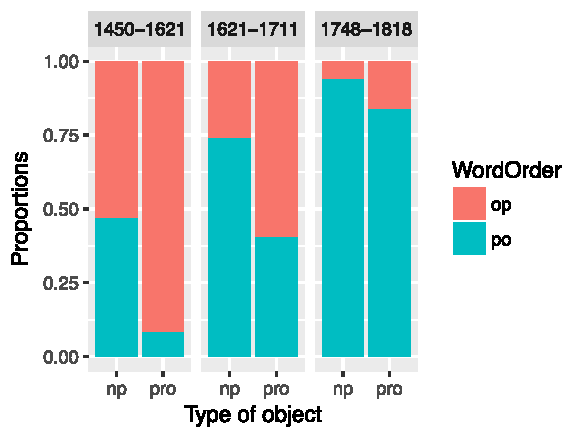
\includegraphics[width=.75\textwidth]{figures/a4-img001.pdf}
\caption{Particle placement with pronominal and non-pronominal objects in three periods. (op = object–particle order; po = particle–object order)\label{fig:lalu:1}} 
\end{figure}


Focusing on individual texts, we note a clear increase in the incidence of the modern word order in the play \textit{Swenska sprätthöken} (1737) by Gyllenborg (born 1679). This text is generally assumed to be a good representative of the spoken language of the upper classes in Central Sweden at the time (see e.g. \citealt{Widmark2000}). From the 18\textsuperscript{th} century onwards, we see effects of style and register in the texts: more conservative texts have more object–particle order, while the development of the particle–object pattern progresses rapidly in the more modern texts. At the end of the century, the modern pattern is almost fully established, for instance in the play by Ristell (born ca. 1750) from 1787. This play can also be considered one of the best sources on the spoken language in Central Sweden at the time. The change is illustrated in \figref{fig:lalu:2}, where we distinguish more modern and more conservative texts. Considering only the texts that we assume best represent the spoken language in Central Sweden at their time, we can observe a cleaner S-shaped curve.


  
\begin{figure}
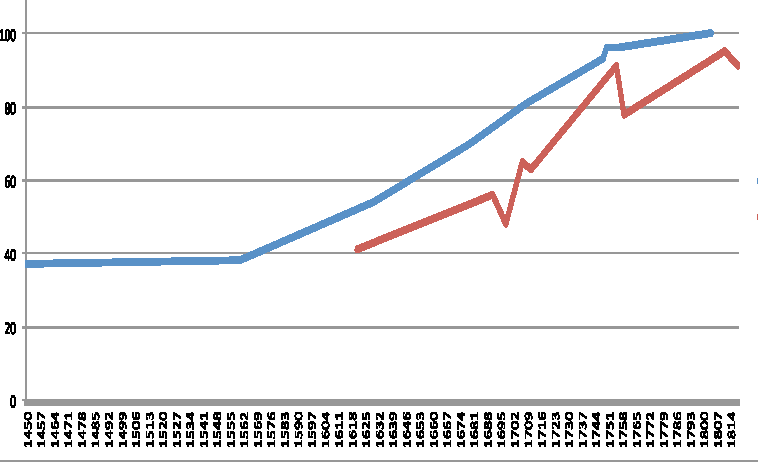
\includegraphics[width=\textwidth]{figures/a4-img002.pdf}
\caption{The development of the order particle–object in more and less conservative texts. The blue line shows texts that are assumed to represent the spoken language of their time. The red line includes more conservative texts.\label{fig:lalu:2}} 
\end{figure}


To summarize, the change can first be observed in the texts by Agneta Horn (b. 1629) and Carl Gyllenborg (b. 1679). This is not unexpected – these are a couple of the historical texts that best represent the spoken language in Central Sweden at their time (as is evident from spelling, morphology, and syntax). The spoken language of Central Sweden is an important source for the modern Swedish standard language (see \citetv{chapters/01}). 


\subsection{Different objects, particles, and contexts}\label{sec:lalu:5.2}

In the development of the modern word order, we can first note a change in the placement of pronominal objects. In the earliest period, there are, as we saw in \sectref{sec:lalu:4} above, only a few examples of pronouns following particles. With a single exception, all of these cases involve either the preposition \textit{till} or ground objects, and they should arguably be treated as involving PPs. In the text by Horn (b. 1629), we find the first clear examples of modern particle order with pronominal objects: clearly non-prepositional particles precede pronominal objects that do not carry the semantic role of ground. In the text by Horn, the order particle–pronoun occurs with all types of particles, unlike in the texts discussed in \sectref{sec:lalu:4.2} above. As in the older texts, objects with the thematic role of ground follow the particle; see \REF{ex:lalu:32a}. In addition, particle verbs like \textit{tycka om} ‘like’ (lit. ‘think about’) and \textit{hålla av} ‘like’ (lit. ‘hold off’) always have the particle before the object. However, we find pronouns following particles in other cases as well; see \REF{ex:lalu:32b} and especially \REF{ex:lalu:32c}, where the internal argument carries the role of figure. However, note that most pronouns (51\%) still precede particles in Horn’s text; one example is given in \REF{ex:lalu:33}. 40\% of the full DP objects have the old word order.


\ea\label{ex:lalu:32}
\ea\label{ex:lalu:32a}
\gll  när   hon   skule     kläda  på   mig\\
    when   she   would   dress    \textsc{part}   me\\
\glt `when she would dress me’ (Horn, b. 1629, p. 38)\\

\ex\label{ex:lalu:32b}
\gll  så   torde     di     inte   häler     så  gå    åt     oss\\
    so   dared   they   not   either   so  go    \textsc{part}   us\\
\glt `so didn’t they dare to get at us so, either’ (Horn, b. 1629, p. 11)\\
\ex\label{ex:lalu:32c}
\gll at       iag   icke   länge   sedan   har   gråtit   vt     dem \\
    that    I     not   long     ago     have   cried     out   them\\
\glt `that I hadn’t long ago cried them [my eyes] out’ (Horn, b. 1629, p. 38)\\
\z
\ex\label{ex:lalu:33}
\gll  Och       toge   de     mig   vp \\
and     took   they   me   up\\
\glt `and they took me up’ (Horn, b. 1629, p. 29)\\
\z


In the 18\textsuperscript{th} century, we find examples of pronouns following non-prepositional particles even in the more conservative texts (by Modée and Salvius); see the examples in \REF{ex:lalu:34} with particle–pronoun order and the examples in \REF{ex:lalu:35} with pronouns preceding particles.


\ea\label{ex:lalu:34}
\ea\label{ex:lalu:34a}
\gll  tvungit   ut   dem\\
   forced   out   them\\
\glt `forced them out’ (Modée, b. 1698)\\

\ex\label{ex:lalu:34b}
\gll  åto  up  dem     så   råa   som  de   voro\\
    ate    up  them    as   raw   as     they   were\\
\glt `ate them up as raw as they were’ (Salvius, b. 1706, chapter 79)\\
\z
\ex\label{ex:lalu:35}
\ea\label{ex:lalu:35a}
\gll  skulle   betala   det   ut\\
    would   pay     it     out\\
\glt `would pay it out’ (Modée, b. 1698)\\

\ex\label{ex:lalu:35b}
\gll  kände     mig   igen \\
   recognize   me   \textsc{part}\\
\glt `recognized me’ (Salvius, b. 1706, chapter 76)\\
\z
\z


We have not systematically investigated the ordering of particles and reflexives; recall from \sectref{sec:lalu:2} that there is still variation in the placement of reflexives in present-day Swedish. However, we can note that from Horn onwards, it is possible to find examples of reflexives following the particle:


\ea\label{ex:lalu:36}
\ea\label{ex:lalu:36a}
\gll  Iag   kune   kläda   på     mig\\
    I        could   dress     \textsc{part}    \textsc{refl} \\
\glt `I could dress myself’ (Horn, b. 1629, p. 65)\\

\ex\label{ex:lalu:36b}
\gll  sedan   vi     hade    väl   friskat     up   oss\\
    as         we    had     well   freshened  up   \textsc{refl}\\
  \glt `as we had freshened up well’(Salvius, b. 1706, chapter 21)\\
\z
\z


The difference between pronominal and non-pronominal objects was retained well into the Late Modern Swedish period. By the beginning of the period, the modern word order was the general rule with non-pronominal objects for some writers. Gyllenborg (b. 1679) has only a few examples of the old order with non-pronominal objects, whereas around half of the pronominal objects are placed before a particle. Examples are given in \REF{ex:lalu:37} and \REF{ex:lalu:38}.


\ea\label{ex:lalu:37}
\ea\label{ex:lalu:37a}
\gll  Binda   dem     up     bakom   öronen\\
    bind     them     up     behind   ears\textsc{.def}\\
\glt `bind them up behind the ears'

\ex\label{ex:lalu:37b}
\gll  om   mina   maner     ej     stå   alla   an \\
    if     my     manners   not   befit   all   \textsc{part}\\
\glt `if my manners do not befit everyone'      (Gyllenborg, b. 1679)\footnote{When referring to texts in the electronic corpus of Swedish drama dialogue, we give only the author and year of birth, not the page number.} \\
\z
\ex\label{ex:lalu:38}
\ea
\gll  Tar   upp   ett   hoprullat   papper\\
    picks     up   a     up-rolled     paper\\
\glt `picks up a rolled-up paper'

\ex
\gll  så    godt   som   kiöra    ut     mig \\
    as    good   as     drive     out   me\\
\glt `as good as expel me’ (Gyllenborg, b. 1679)\\
\z
\z


We can also note that Olof von Dalin, who is often taken to mark the introduction of the new period (see \citetv{chapters/01}), only has one example with a non-pronominal object in the old word order; it is given in \REF{ex:lalu:39}.


\ea\label{ex:lalu:39}
\gll  om   wåra   förfäder       skulle   nu   sätta   sina   hufwuden   upp\\
if     our     forefathers     would   now   put   their     heads     up\\
\glt `if our forefathers would now put their heads up’ (Dalin, b. 1708)\\
\z


Note that the particle in \REF{ex:lalu:39} is an adverb. This does not appear to be a coincidence. Rather, it seems that word order variability remained somewhat longer with adverbs than with prepositions. In fact, all examples of the old word order with non-pronominal objects in the text by Horn have either an adverb or involve the preposition \textit{till} with a benefactive object; see \REF{ex:lalu:40a} and \REF{ex:lalu:40b}. Examples like \REF{ex:lalu:41}, from the older text by Kiöping, with other prepositional constructions combined with non-pronominal objects, are completely missing from Horn’s text.


\ea\label{ex:lalu:40}
\ea\label{ex:lalu:40a}
\gll  Skulle  han   lösa     sin         fas       hus in\\
    would  he   redeem   \textsc{poss.refl}   father’s   house   \textsc{part}\\
\glt `would he redeem his father’s house’ (Horn, b. 1629: 52)\\

\ex\label{ex:lalu:40b}
\gll  skrifwit   min   h[är] f[ar] til\\
    written   my   sir   father   to \\
\glt `written to my father’ (Horn, b. 1629, p. 49)\\
\z
\ex\label{ex:lalu:41}
\ea
\gll  Sedan   taga   the     Blyringarna     aff\\
    then     take   they   lead.ring.\textsc{pl.def}   off\\
\glt `then they take off the lead rings’ (Kiöping, b. 1621, p. 98)\\

\ex
\gll  Måste   sluta     alla   wåra   lukor     till \\
    must     close     all   our   hatches   \textsc{part}\\
\glt `must close all our hatches’ (Kiöping, b. 1621, p. 44)\\
\z
\z


In \sectref{sec:lalu:4.2} above, we saw that objects always precede directional adverbs followed by PPs in the three oldest texts in the corpus. This is still the case in the text by Horn; see \REF{ex:lalu:42}.


\ea\label{ex:lalu:42}
\gll  kasta     mig   in     til     fru     eba\\
threw       me   in     to     Madam   Ebba\\
\glt `threw me in to Madam Ebba’(Horn, b. 1629, p. 13)\\
\z

\begin{sloppypar}
The first clear examples in the corpus of particles preceding object\,+\,directional PP are found in the text by Salvius from 1743; see \REF{ex:lalu:43}. Here, we see a clear difference between the Late Modern Swedish text and the earlier version of the same text by Kiöping; cf. \REF{ex:lalu:25b} above.
\end{sloppypar}

\ea\label{ex:lalu:43}
\gll  De {fiska} {hvar}     {dag} \textbf{up} \textit{pärle} \textit{skal} {af} {botnen} {til} {största} {myckenhet}\\
they   fish     every   day     up     pearl   shells   of     bottom\textsc{.def} of     largest     quantity\\
\glt `Every day they fish up the largest quantity of pearl shells from the bottom'   (Salvius, b. 1709, chapter 72)\\
\z

\begin{sloppypar}
In the 18\textsuperscript{th} and 19\textsuperscript{th} centuries, there is still variation in these contexts. Even in the youngest text in the corpus, there are examples of the order object–particle\,+\,PP, where present-day Swedish would require a different word order. One such example is given in \REF{ex:lalu:44}.
\end{sloppypar}

\ea\label{ex:lalu:44}
\gll  lägger   några   vedträn   som   legat   framför       kaminen in       i     densamma\\
puts       some     logs     that     lain     in.front.of   stove.\textsc{def} in   to   the.same\\
\glt `puts some logs that have lain in front of the stove into it’ (Jolin, b. 1818)\\
\z


In addition to the directional particles followed by PPs, there is one other type of context where the old word order is retained, namely where present-day Swedish no longer has a construction with a free particle. For instance, the example in \REF{ex:lalu:37b} involves the particle \textit{an}; in present-day Swedish, \textit{an} would have been prefixed (\textit{anstå} ‘befit’). Similar examples are given in \REF{ex:lalu:45}. It seems that these elements often lack the typical semantic characteristics of verb particles: they do not introduce an endpoint or a figure argument; see e.g. the stative VP in \REF{ex:lalu:45c}.


\ea\label{ex:lalu:45}
\ea\label{ex:lalu:45a}
\gll  Och   gaf   mig     inte     öfwer   för     någet       litet\\
    and     gave  me   not   \textsc{part}     for     something   small\\
\glt `and didn’t abandon me for a small thing’ (Horn, b. 1629: 24)\\
    Present-day Swedish: \textit{övergav}\\

\ex\label{ex:lalu:45b}
\gll  så    godt   som   för   ingen ting   falla   en  ährlig   Karl   til \\
    so     good   as     for   nothing     fall   an  honest   man   \textsc{part}\\
    ‘is passed on to an honest man for almost nothing’ (Modeé, b. 1678)\\
    Present-day Swedish: \textit{tillfalla} \\
\ex\label{ex:lalu:45c}
\gll hör       mig   ej     mera   till \\
    belong   me   not   more   \textsc{part}\\
\glt `no longer belongs to me’ (Enbom, b. 1759)\\
    Present-day Swedish: \textit{tillhör}\\
\z
\z


To sum up, we can identify three stages in the development of the Swedish word order in particle constructions:


\begin{description}
\item[Pre-change (–1629):] Light pronouns obligatorily precede particles, while full DP objects either follow or precede particles. Examples with ground objects or with a PP should not be included among the particle constructions.
\item[Change (authors born 1629–1711):] In the text by Horn (b. 1629) we find the first clear instances of particles preceding pronominal (and sometimes reflexive) objects. The frequency of the order particle--object increases rapidly, but object–particle order is still common, especially with pronouns.
\item[Post-change (authors born 1748–1818):] In the texts by authors born after 1748 (i.e., texts from the late 18\textsuperscript{th} century onwards) we find a system that looks like the present-day Swedish system, with particles more or less obligatorily preceding objects. We still find at least two more or less systematic types of counterexamples: 1) particles appearing together with directional PPs, and 2) particles with atypical semantics, i.e. that neither provide an endpoint nor take a figure external argument (see \REF{ex:lalu:45}).
\end{description}

In \sectref{sec:lalu:7}, we discuss changes that may have taken place more recently.


\section{Discussion}\label{sec:lalu:6}


As stated in \sectref{sec:lalu:2.2} above, the empirical investigation of particles in the historical texts started with a rather liberal definition of \textit{particle}. Among other things, we included particle-like elements combined with a PP, although they sometimes seem to form a constituent with the PP in present-day Swedish. Moreover, we included examples with objects that have the semantic role of ground, as opposed to the prototypical figure role of arguments of particles. As noted, these particles do not seem to behave like particles with respect to word order in, for instance, present-day Norwegian.



By including the less typical cases, we can investigate what should be included in the particle category in older Swedish. In fact, we find that the category is not historically completely stable. Firstly, the cases with a prepositional element\,+\,a ground object do not behave like particle constructions in the older texts, but rather seem to pattern with PPs. This also includes the examples with \textit{slå till} ‘strike,’ although, in this case, it is less clear that the object is a ground than in the examples with a locative meaning. Secondly, examples with an adverb followed by a PP do not behave like particle constructions either, at least not until the middle of the 18\textsuperscript{th} century; here, the order object–particle is obligatory in the older texts, and it has continued to be a possibility even into the present day. We propose that the particle here is best analyzed as part of the PP in older Swedish, but that it has been reanalyzed as a regular verb particle; we return to this below. Finally, there are cases where what seems to be a particle in older Swedish no longer is. In present-day Swedish, these cases are either verbal prefixes (e.g. \textit{stå an} – \textit{anstå} ‘befit’) or have completely disappeared from the language. In many cases, the particle-like element does not have the resultative semantics typical of verb particles. 



In addition to the changes in what is included in the particle category, we can identify three separate (but related) word order changes: 1) the emergence of particles preceding light pronominal objects; 2) the establishment of a categorical particle–object order in constructions without a directional PP, and 3) a change in the word order in constructions with particle\,+\,PP. Related to the last point, we also believe that there has been a more recent development, where the frequency of modified particles (e.g. \textit{throw the stone far out}) has decreased. We return to this in the concluding section of the chapter.



In this section, we discuss possible analyses of these changes. We will in turn look at what we see as the two main alternatives. Firstly, one could analyze the change in particle constructions as being on a par with the change from OV to VO order, i.e. either as a consequence of the headedness of the particle or in terms of argument shifts across the particle head (as suggested for the development of VO order, e.g. by \citealt{Petzell2011}). In an account along such lines, the word order change in particle constructions would be another step toward a consistent head-initial language. An alternative is to assume that Swedish particles have become different, and that the word order change is a consequence of a reanalysis of the particle. 



In the following, we discuss these two possibilities in turn. In \sectref{sec:lalu:6.1}, we briefly compare the word order change in particle constructions with the change from OV order to VO order. Although this alternative might seem initially appealing, we will see that it is problematic to assume object movement across a verb phrase-internal head in 17\textsuperscript{th} and 18\textsuperscript{th} century Swedish. Moreover, the analysis fails to account for the parallels between older Swedish and present-day Norwegian. In \sectref{sec:lalu:6.2}, we look more closely at pronominal argument shifts in older Swedish, and we observe that the word order change in Early and Late Modern Swedish is limited to constructions with a particle: object shift across negation is not affected. Finally, in \sectref{sec:lalu:6.3}, we will propose that the observed changes in particle constructions are best understood as resulting from one single underlying change: a reanalysis of particles from phrasal modifiers to heads in the verb phrase. By assuming that the particle was a phrase in older Swedish, we can more straightforwardly explain the word order variation. At the same time, this allows us to account for other changes in the properties of particles that took place during the same period, e.g. the loss of the possibility to combine adverbial particles with a double object structure. Finally, the more recent change in constructions with particle\,+\,PP follows from the same underlying change: in older Swedish, the particle modified the PP, whereas in present-day Swedish, there is a strong preference for treating the particle as a head. We will tentatively suggest that this also accounts for a drop in the use of modified particles.


\subsection{OV to VO and OP to PO}\label{sec:lalu:6.1}

The shift to strict particle–object order partly overlaps with the shift from OV order to VO order. The change from OV to VO had mainly taken place during the 13\textsuperscript{th} century (see e.g. \citealt{Delsing1999}), but OV structures increased in the late 15\textsuperscript{th} century, and residual OV word order is not hard to find in the 16\textsuperscript{th} and 17\textsuperscript{th} century texts. It is perhaps tempting to view the two changes as one and the same, i.e., as a shift to a consistent head-initial word order. 



In fact, the two changes share some characteristics, most notably that pronouns seem to stick to the old patterns longer than fully fledged DPs. \citet[174]{Delsing1999} notices that after 1375, the attested OV patterns usually have pronominal objects (but not just personal pronouns), or bare NP objects, that seem to form a complex event with a light main verb (presumably not very different from a particle structure). However, even in the medieval laws, OV is not completely obligatory with pronominal objects, but occurs in around 70–80\% of the cases (see \citealt{Delsing1999}, \tabref{tab:lalu:2}). Object–particle order with pronominal objects, in contrast, seems to have been fully obligatory until the late 16\textsuperscript{th} century. In the time period when the word order in particle constructions began to change, several types of OV structures can be found. The object could either appear to the left of a verb complex consisting of a finite verb and one or several non-finite verbs, or directly to the left of the main verb (see \citealt{Petzell2011, Petzell2012, Petzell2011}). During the 16\textsuperscript{th} century, there was an increase in structures with non-finite verbs preceding the finite verb, presumably arising from German influence.



The OV-to-VO change has been analyzed in at least two different ways that in principle could be generalized to the shift from object–particle (OP) to particle–object (PO) order: 


\begin{itemize}
\item There was a change in a headedness parameter: whereas both verb phrases and particle phrases were originally head-final, at a later stage, both vP/VP and ParticleP became head-initial.
\item The possibility of vP-internal argument shift became more restricted over time, i.e., landing sites for arguments inside the vP disappeared, leading to both VO and PO orders.
\end{itemize}

With regard to particles, both of these options turn out to be problematic from a comparative perspective: all the North Germanic languages and English lost the OV order centuries ago, but only Swedish developed a strict ordering of objects and particles. The stable variation found in Icelandic, Norwegian, and English (which looks much like the variation in older Swedish) can hardly be accounted for in terms of headedness. We will therefore not pursue that possibility further, but still briefly discuss the correlation between OV-to-VO and OP-to-PO expected from the second option.



OV structures in older Swedish have been analyzed as DP movement from a low VP position (the complement of V) to a higher specifier inside the extended verb phrase (\citealt{Delsing1999}; \citealt{Petzell2011, Petzell2012, Petzell2011}). In principle, the same account could be given for the old object–particle order: object–particle orders can be treated as a residue of OV, where the object lands in a low specifier position (possibly of the particle). In \REF{ex:lalu:46} below, we give three possible landing sites for the objects, corresponding to the specifier of the particle, the main verb, and the finite auxiliary (or possibly an even higher specifier), respectively.\footnote{\citet{Petzell2012} analyses the German-like order Object–Main Verb–Finite Aux as a result of pied-piping of the main verb by the object.

    \ea
    \gll  Eftersom    han [[hunden   sälja [hunden]]   ska [[hunden]   sälja   hunden].\\
    since   he     dog.\textsc{def}   sell       dog.\textsc{def}     will   dog.\textsc{def}     sell   dog.\textsc{def}\\
    \z}


\ea\label{ex:lalu:46}
\gll Eftersom  han <\textsubscript{3} hunden>   ska   <\textsubscript{2} hunden> kasta     <\textsubscript{1} hunden>   ut     hunden.\\
since        he      dog\textsc{.def}  will     dog\textsc{.def}  throw        dog\textsc{.def}   out   dog\textsc{.def}  \\
\z


In \tabref{tab:lalu:3} below, we compare the proportion of particle–object order (PO) to the proportion of VO in four texts (where we have access to the VO data, from \citealt{Petzell2012}). Although the proportions of both VO and PO increase over time, as seen in \tabref{tab:lalu:3}, the shift to VO order is, as expected, earlier than the establishment of the strict PO order. Specifically, we see clearly different proportions for PO and VO for pronouns in the last text in the sample \citep{Salvius1706}, which suggests that the OP order was freely available, and maybe even preferred, at a stage where other VP-internal shifts were rarely available.


\begin{table}
\caption{The frequency of particle–object and verb–object order in four Modern Swedish texts. (The number of examples is given in parentheses.) The data on VO order is taken from \citet{Petzell2012}.}
\label{tab:lalu:3}
\begin{tabularx}{0.85\textwidth}{Xrrrr}
\lsptoprule
& PO, pro & VO, pro & PO, DP & VO, DP\\
\midrule
Swart (1560) & 11.5\%(26) & 40\%(10) & 47\% (74) & 72.7\% (11)\\
Kiöping (b. 1621) & 3.7\% (27) & 40\% (45) & 58\% (43) & 62\%   (37)\\
Horn (b. 1629) & 49.2\%   (69) & 53\%   (88) & 60\% (58) & 88.6\% (35)\\
Salvius (b. 1706) & 18.7\%(32) & 73\%(23) & 80\% (82) & 96.8\% (31)\\
\lspbottomrule
\end{tabularx}
\end{table}

We could in principle assume that Swedish lost its landing positions within the verb phrase gradually, and that the lowest ones were available the longest. This would mean that the other North Germanic languages (and English) kept a low landing position in the verb phrase, a position either headed by or modified by the particle. There is one crucial problem with such a proposal, and that concerns regular object shift.\footnote{Erik Petzell (p.c.) points out that there is another problem with such a proposal, namely that in the loss of OV order, short movement of the object (giving the order V\textsubscript{aux}–object--V\textsubscript{main}) seems to disappear before long movement (giving the order object--V\textsubscript{aux}–V\textsubscript{main}); see \citet{Petzell2012}.} A well-known difference between particles in Swedish and the other North Germanic languages is that particles block object shift in Swedish, but not in the other languages (see e.g. \citealt{Holmberg1986}; \citealt{Sells1998}). In Swedish, a particle behaves just like a verb inside the verb phrase; compare \REF{ex:lalu:47a} with \REF{ex:lalu:47b} and \REF{ex:lalu:47c}.


\ea\label{ex:lalu:47}
\ea\label{ex:lalu:47a}
\gll  Jag   kastade   den   inte.\\
 I       threw   it     not\\
\glt `I didn’t throw it.'

\ex\label{ex:lalu:47b}
\gll Jag    har   \{*den\}  inte   \{*den\}   kastat   \{den\}.\\
    I       have     it    not     it     thrown     it\\
\glt `I haven’t thrown it.’\\
\ex\label{ex:lalu:47c}
\gll Jag  kastade   \{*den\}   inte   \{*den\}   ut     \{den\}.\\
    I     threw       it      not     it      out     it      \\
\glt `I didn’t throw it out.'
\z
\z


\REF{ex:lalu:47a} illustrates object shift: when the verb has moved out of the verb phrase, a light pronominal object can shift across the sentence adverbial. If the verb remains in the VP, object shift is impossible, as seen in \REF{ex:lalu:47b}; this is often referred to as Holmberg’s generalization (after \citealt{Holmberg1986}). In \REF{ex:lalu:47c}, the verb has moved out of the VP, but object shift is still impossible: it is blocked by the particle.



The restrictions on pronominal object shift are the same in Swedish as in the other North Germanic languages, with the exception of shift across particles. In the other North Germanic languages (exemplified with Norwegian in \REF{ex:lalu:48}), a light object pronoun must shift across both the particle and the sentence adverb (in the context of verb movement). Swedish seems to have been like present-day Norwegian up until the 18\textsuperscript{th} century (although the relevant examples are few); see the examples in \REF{ex:lalu:49}.


\ea\label{ex:lalu:48}
\gll Jeg  kastet \{den\}     ikke   \{*den\}   ut   \{*den\}      (Norwegian)\\
I       threw   it      not       it      out         it\\
\glt `I didn’t throw him out yesterday'
\ex\label{ex:lalu:49}
\ea
\gll  Män   thet   går           henne   inte     an\\
    but       it    concerns   her   not     \textsc{part}\\
  \glt `but it doesn’t concern her’ (Horn, b. 1629, p. 55)\\

\ex
\gll  känner     du   mig     inte     igen \\
    recognize   you   me     not     \textsc{part}\\
\glt `don’t you recognize me’ (Modeé, b. 1698)\\
\z
\z


It is unclear why a VP-internal landing site, e.g. in the specifier of a particle phrase, would be required for the pronominal object to shift into the TP. Compare this with object shift in the context of a verb without a particle, where we standardly assume that the object moves directly from an internal argument position to TP, independent of the presence of landing sites within the VP. Rather, the literature on contemporary North Germanic object shift (e.g. \citealt{Thrainsson2001}) shows that it is impossible to shift over overt heads, as exemplified with a verbal head in \REF{ex:lalu:47b} above and a prepositional head below:


\ea\label{ex:lalu:50}
\ea
\gll Jag  ska  \{*den\}   inte   köpa   \{den\}   imorgon.\\
      I         will      it      not  buy     it     tomorrow \\
\glt  ‘I will not buy it tomorrow'

\ex
\gll Jag  litar   \{*honom\}   inte   på   \{honom\}.\\
    I     trust     him     not   on     him\\
\glt  ‘I don’t trust (on) him'
\z
\z


This suggests that object shift in the present-day North Germanic languages is qualitatively different from the movement of objects around verbs in earlier OV stages. On the other hand, the obligatory shift of light pronominal objects around particles in older Swedish (and in present-day Norwegian and Icelandic) looks more like typical object shift. 



In the next section, we take a closer look at pronominal object shift in our historical corpus and compare it to the placement of objects relative to particles. We will suggest that the well-established generalization that pronouns do not move across heads should also be maintained for particle constructions in the present-day North Germanic languages. This means that the particle is not a head, for instance, in present-day Norwegian. Rather, it is a phrasal modifier of a resultative phrase low in the verbal domain. We propose that this was the case in Swedish as well, up until the middle of the 17\textsuperscript{th} century, and that the particle was then reanalyzed as a head. 


\subsection{Pronominal object shift and word order variation in particle constructions}\label{sec:lalu:6.2}

Present-day Swedish differs from present-day Danish and (varieties of) Norwegian in the optionality of pronominal object shift: whereas light pronominal objects obligatorily shift around negation and other sentence adverbs in the contexts of V-to-C movement in Danish and Norwegian, this shift appears to be optional in Swedish (see \citealt{Bentzen2014} and references therein); compare the present-day Swedish example in \REF{ex:lalu:51a} with the Norwegian example in \REF{ex:lalu:51b}. In the Swedish data in the Nordic Word Order database \citep{LundquistEtAl2019}, 30\% (144/478) of the pronominal objects are \textit{not} shifted but follow negation. In corpus data, around 90\% of pronouns with nominal antecedents shift in Swedish (see e.g. \citealt{Andreasson2008}); pronouns with non-nominal antecedents or type reference shift less frequently.


\ea\label{ex:lalu:51}
\ea{\label{ex:lalu:51a}
\gll Jag  köpte \{den\}  inte \{den\}   igår.\\
    I       bought   it      not     it       yesterday\\\jambox*{(present-day Swedish)}
  \glt `I didn’t buy it yesterday'}

\ex{\label{ex:lalu:51b}
\gll Jeg  kjøpte   \{den\}  ikke \{*den\}  igår.\\
    I     bought     it      not       it     yesterday\\\jambox*{ (Norwegian)}
  \glt `I didn’t buy it yesterday'}
\z
\z


We have investigated the placement of object pronouns and reflexives in relation to negation in the 18 texts in our historical corpus; the results are given in \tabref{tab:lalu:4}. Reflexives have been included here, since they shift in the same way as weak pronouns, but we have excluded 41 pronouns with non-nominal antecedents entirely, since they show a different pattern (with only 37\% object shift in this corpus). On the other hand, we have included possibly contrasting pronouns with nominal reference, and they account for almost all of the examples with non-shifted pronouns.


\begin{table}
\caption{Placement of personal object pronouns and reflexives relative to negation in older Swedish.}
\label{tab:lalu:4}
\begin{tabular}{lcc}
\lsptoprule
Text & Pronoun–negation & Reflexive--negation\\
\midrule
\textit{Didrik} (ca. 1450) & 10/10 & 1/1\\
\citet{Swart1560} & 10/10 & 5/6\\
Kiöping (b. 1621) & 5/5 & 6/6\\
Horn (b. 1629) & 28/29 & 7/7\\
Gyllenborg (b. 1679) & 11/12 & 5/5\\
Lagerström (b. 1691) & 10/12 & 17/19\\
Modée (b. 1698) & 16/17 & 21/21\\
Salvius (b. 1706) & 2/2 & 2/2\\
Dalin (b. 1708) & 8/10 & 4/4\\
Stagnell (b. 1711) & 4/4 & 1/2\\
Kexél (b. 1748) & 3/4 & 2/2\\
Ristell (b. ca. 1750) & 3/4 & 4/6\\
Stridsberg (b. 1755) & 7/7 & 6/6\\
Envallsson (b. 1756) & 8/12 & 4/4\\
Enbom (b. 1759) & 11/13 & 3/5\\
Wetterbergh (b. 1804) & 6/6 & 4/4\\
Blanche (b. 1811) & 2/2 & 2/2\\
Jolin (b. 1818) & 17/19 & 1/3\\
\midrule
Total & 161/178 (90\%) & 96/105 (91\%)\\
\lspbottomrule
\end{tabular}
\end{table}

It seems clear from the results in \tabref{tab:lalu:4} that pronominal object shift is (almost) obligatory in older Swedish; as many as 90\% of the pronouns shift across negation. Although the number of examples is small in the individual texts, we can conclude that the placement of pronouns in relation to negation is stable during the period.



There are, as we saw in \sectref{sec:lalu:4} above, only a few examples of pronouns following particles in the oldest texts in the corpus. With a single exception, all these cases involve either the preposition \textit{till} or ground objects, and they should arguably be treated as involving PPs. In these texts, object shift also appears to be obligatory (although the examples are few). However, unlike what we saw with the order of particles and pronouns, there was no general increase in the frequency of the order negation–pronoun in the 17\textsuperscript{th} century. Recall that we find the first clear examples of modern particle order with pronominal objects in the text by Horn. In principle, this order could be seen as just an absence of object shift around the particle. However, there is otherwise nothing particularly unusual about Horn’s placement of pronominal objects. Notably, she consistently shifts pronominal objects around negation, with a single exception, and there, the pronoun is contrasted; see \REF{ex:lalu:52}.


\ea\label{ex:lalu:52}
\gll  När       han  gaf   hene   någet,       sade   iag:   Hwar före gefwa   i     inte   mig   och\\
when    he   gave   her   something   said   I       why   give     you   not   me   too\\
\glt `When he gave her something, I said: Why don’t you give me, too’ (Horn, b. 1629, p.~78)\\
\z


Before the middle of the 17\textsuperscript{th} century, the placement of pronouns in relation to particles patterned with object shift, and we could in principle treat particles as regular adverbs. However, from Horn onwards, such an analysis is no longer possible. The data in \tabref{tab:lalu:4} strongly suggest that the change in particle–pronoun placement is not related to changes in general object shift.



We propose that the order pronoun–particle in older Swedish (up until the middle of the 17\textsuperscript{th} century) and present-day Norwegian should be treated together with object shift, and that the placement of pronouns and DPs was regulated by different mechanisms in earlier stages of Swedish. We suggest the following analysis: the figure argument is the specifier of the result phrase.\footnote{Note that the figure argument will be promoted to subject if the verb is intransitive, as in e.g. \textit{Maria dansade in i rummet} (‘Maria danced into the room’), where Maria is the figure.} At earlier stages, the particle was merged as a light phrasal modifier of ResP, and could either surface to the left or the right of the specifier, which for simplicity we will state in terms of the branching directionality of the modifier. The pronominal object always shifts past the phrasal modifier, a movement/shifting operation that is identical to regular object shift (which can be stated either as a syntactic movement, or as PF cliticization of a light pronoun to a non-adverb element). 



We illustrate the options in the tree structures below, which provide possible derivations of (the correspondences of) \textit{Kalle threw out the dog} and \textit{Kalle threw it out} in older Swedish. Firstly, in \REF{ex:lalu:53a}, the adjunct of ResP branches to the left, and will therefore linearly precede the object DP. If the object is a pronoun, it shifts to a higher specifier in the VP (here, spec-VP) and will precede the particle. In \REF{ex:lalu:53b}, the adjunct branches to the right, and both DP and pronominal objects will precede the particle.


\ea\label{ex:lalu:53}
\ea\label{ex:lalu:53a}
% \includegraphics[width=\textwidth]{figures/a4-img003.tif}
\begin{forest}
  [vP
    [DP
        [Kalle]
    ]
    [vP
        [v
            [kasta]
        ]
        [VP
            [Pron.
                [den]
            ]
            [VP
                [V
                    [\sout{kasta}]
                ]
                [ResP
                    [PartP
                        [ut]
                    ]
                    [ResP
                        [DP
                            [hunden/\sout{den}]
                        ]
                        [Res
                            [$\emptyset$]
                        ]
                    ]
                ]
            ]
        ]
    ]
  ]
\end{forest}


\ex\label{ex:lalu:53b}
% \includegraphics[width=\textwidth]{figures/a4-img004.tif}
\begin{forest}
  [vP
    [DP
        [Kalle]
    ]
    [vP
        [v
            [kasta]
        ]
        [VP
            [Pron.
                [den]
            ]
            [VP
                [V
                    [\sout{kasta}]
                ]
                [ResP
                    [ResP
                        [DP
                            [hunden/\sout{den}]
                        ]
                        [Res
                            [$\emptyset$]
                        ]
                    ]
                    [PartP
                        [ut]
                    ]
                ]
            ]
        ]
    ]
  ]
\end{forest}
\z
\z



The branching alternation we see above, we suggest, is similar to that of light temporal and spatial adverbs that may left- or right-adjoin to the vP, either preceding the whole vP-internal cluster of verbs \REF{ex:lalu:54a}, or following the whole vP \REF{ex:lalu:54b}, but never appearing inside the verb cluster:


\ea\label{ex:lalu:54}
\ea\label{ex:lalu:54a}
\gll  Kalle  borde   idag     ha     kastat   ut     hunden.\\
    Kalle   should   today   have   thrown   out   dog\textsc{.def}\\
\glt `Kalle should have thrown out the dog today.'

\ex\label{ex:lalu:54b}
\gll  Kalle   borde   ha   kastat   ut     hunden   idag.\\
 Kalle   should   have   thrown   out   dog\textsc{.def}   today\\

\ex
\gll  Kalle   borde   ha   (*idag)     kastat   (*idag)  ut     (*idag)    hunden.\\
    Kalle   should   have   ~~today   thrown   ~~today  out     ~~today   dog\textsc{.def}\\
\z
\z



Now, present-day Swedish is different, and we have argued that the change should not be understood as a change in branching or argument shifts. Instead, we propose that the particle has been reanalyzed as the head of the Result phrase; the structure is given in \REF{ex:lalu:55}.


\ea\label{ex:lalu:55}

\begin{forest}
  [vP
    [DP
        [Kalle]
    ]
    [vP
        [v
            [kasta]
        ]
        [VP
            [Pron.
                [den]
            ]
            [VP
                [V
                    [\sout{kasta}]
                ]
                [ResP
                    [DP
                        [hunden/\sout{den}]
                    ]
                    [Res
                        [ut]
                    ]
                ]
            ]
        ]
    ]
  ]
\end{forest}

% \includegraphics[width=\textwidth]{figures/a4-img005.tif}
\z
 



However, a standard minimalist/generative framework with an LCA-based \citep{Kayne1994} spell-out procedure will not directly be able to capture why the reanalysis led to a categorical change in word order. In \REF{ex:lalu:55}, it might appear as if the particle should end up at the end of the sentence, i.e. after both DPs and pronouns. However, we will build on Mirror Theory, as originally formulated by \citet{Brody2000}, and developed e.g. in \citet{AdgerEtAl2009}, \citet{Ramchand2014}, and \citet{Svenonius2016}, and assume that specifiers and heads are linearized independently of each other. The heads in the clausal spine form a span, which is spelled out at a given point in the tree. In Swedish, we assume this point to be v, as indicated by the @ sign in \REF{ex:lalu:56} below. In the tree in \REF{ex:lalu:56}, the span of heads will spell out directly after the syntactic subject.\footnote{The
    subject will generally move to a higher position, but when it doesn’t (as in existential constructions), it surfaces after the particle, as in (i).

    \ea
    \gll Det   har   aldrig   stått   ut någon   med   det.\\
    it   has  never  stood  out  anyone  with  that‘\\
    \glt No one has ever endured that.’
    \z
} The presence of only one spell out point in the span of heads ensures that all heads are spelled out in the same position with respect to specifiers.


\ea\label{ex:lalu:56}
% \includegraphics[width=\textwidth]{figures/a4-img006.tif}
\begin{forest}
  [(v)@
    [DP
        [Kalle]
    ]
    [(V) kasta
        [Pron.
            [den]
        ]
        [(Res)~ut
            [DP
                hunden/\sout{den}
            ]
        ]
    ]
  ]
\end{forest}

\z

In Swedish, we can state that the heads in the vP cluster up in a left-right order at the left edge of the vP. Verbs in Swedish today form a cluster, in which nothing generally intervenes (of course, here we exclude V in C):


\ea\label{ex:lalu:57}
\gll  Eftersom  Kalle    förmodligen  snart  redan    borde  ha    kunnat kasta     ut   hunden…\\
since         Kalle    probably     soon     already   should  have   been.able.to throw   out  dog\textsc{.def}\\
\z


We will leave a full technical account aside here. In the next section, we will briefly look at a couple of other consequences of the reanalysis of the particle. 


\subsection{Phrase to head}\label{sec:lalu:6.3}

In the previous sections, we have pointed out some problems with directly linking the change in particle placement to a change in the available argument positions in the verb phrase and object shift. Instead, we have proposed that the word order change in particle constructions in Swedish should be understood as a consequence of a reanalysis of particles from phrases to heads: Swedish particles have been reanalyzed from phrasal modifiers of ResP to Res heads. Since the heads in the verb phrase are linearized together before arguments and adjuncts in Late Modern Swedish, the reanalysis leads to the fixed modern word order. 



This means that the change is another example of the Head Preference Principle (\citealt{van_Gelderen2004}) at work. This principle states that when there is no evidence to the contrary, a word will be analyzed as a head rather than a phrase. \citet{van_Gelderen2004} introduces this principle as one of several economy principles which are part of universal grammar and guide children’s acquisition of a language. The principle has previously been invoked to account for the reanalysis of negation (see e.g. \citealt{Van_gelderen2008}) and the loss of V2 order with certain question words in varieties of Norwegian \citep{WestergaardEtAl2017}.\footnote{Other similar principles have also been proposed, e.g. \textit{Minimize structure} (\citealt{CardinalettiStarke1999}; \citealt{BreitbarthEtAl2020}). In the present context, nothing hinges on the precise formulation of the economy principles.}  



We can identify two stages in the change. Firstly, there is stage at which particles start to behave like heads. This stage can be identified by the possibility of unambiguous particles that precede light pronominal objects, as first observed in the text by Horn from the middle of the 17\textsuperscript{th} century. As discussed above, the assumption is that weak pronouns obligatorily shift across adverbial phrases, including both negation and the older phrasal particles, but that they cannot shift across a head. In the second stage, the particle has to fill the Res head, and the modern word order becomes obligatory. 



In this analysis, the word order change is tied to a reanalysis of the particle. In fact, we can note a couple of other changes that occurred around the same time, which arguably are also a consequence of the change in the syntax of particles. Firstly, in older Swedish, adverbial particles could occur in double object constructions, as in \REF{ex:lalu:58}. This is no longer possible in present-day Swedish, regardless of word order; compare \REF{ex:lalu:59} and \REF{ex:lalu:60}.


\ea\label{ex:lalu:58}
\ea
\gll  så   ge     mig     hit  en   skål  \\
 so   give     me     here   a     bowl \\
\glt `so give me a bowl here’ (Gyllenborg, b. 1679)\\

\ex
\gll  torde  jag […]  kunna     betala   den   Narrn     sin   fulla   lön   ut \\
      ought  I   {}    be.able.to  pay     the   fool\textsc{.def}   his   full   salary   out\\
\glt `I ought to be able to pay the fool his full salary’ (Modée, b. 1698)\\
\z
\ex\label{ex:lalu:59}
\ea{
\gll  Ge     mig (*    hit)     en   skål.     \\
    give     me   {}    here   a     bowl\\}\jambox*{(present-day Swedish)}

\ex
\gll  Jag   betalar   honom   (*ut)   hans   fulla   lön.  \\
    I       pay     him       ~~out   his   full   salary\\
\z
\ex\label{ex:lalu:60}
\ea[*]{
\gll    Jag   betalar   ut     honom   hans   fulla   lön. \\
        I       pay     out   him    his     full   salary\\
}
\ex[*]{
\gll   Jag   betalar     honom   hans   fulla   lön ut. \\
        I     pay       him    his   full   salary  out\\
}
\z
\z


This restriction can be explained by the assumption that the head responsible for the introduction of indirect objects competes for the same position (i.e., Res) as the present-day Swedish particle (see e.g. \citealt{Ramchand2008}).



Moreover, in the 18\textsuperscript{th} century, particle incorporation became obligatory in constructions with past participles. Although examples are admittedly rare, cases like those in \REF{ex:lalu:61} can be found in the 16\textsuperscript{th} and 17\textsuperscript{th} centuries. From the 18\textsuperscript{th} century onwards, particles always incorporate into participles (see \citealt{Lundquist2014Passives}); see \REF{ex:lalu:62}.


\ea\label{ex:lalu:61}
\ea[]{
\gll  bleff […]   förd       vth   till   galgan\\
       was    {}  taken     out   to     gallows\textsc{.def}\\
\glt `was taken out to the gallows’ (Swart, 1560, p. 40)\\}

\ex[]{
\gll  blef   sat     in   i   kiörkan       den   sama     hösten \\
    was   put   in   to   church.\textsc{def}     the   same     fall.\textsc{def}\\
\glt `was put in the church the same fall’ (Horn, b. 1629, p. 14)\\}
\z
\ex\label{ex:lalu:62}
\ea[]{
\gll  blev   in-satt   i   kyrkan (present-day Swedish)\\
    was     in-put   in   church\textsc{.def} \\
    }
\ex[*]{
\gll   blev   satt   in   i   kyrkan    \\
        was   put   in   to   church\textsc{.def}\\
        }
\z
\z


Leaving the analysis of particle incorporation aside, we conclude that there are several reasons to assume that the word order change is a consequence of a change in the syntax of particles, rather than, for instance, in the general principles of linearization in Swedish or the possibility of argument shifts. 



While we find the first evidence for particles as heads in the middle of the 17\textsuperscript{th} century, it took considerable time before the Res head was obligatorily filled. We saw in \sectref{sec:lalu:5} above that the preference for particles in Res depends partly on the type of element and the context. Prepositions were generally affected before adverbs, and in the context of a PP, the adverb was often a phrasal modifier well into the 19\textsuperscript{th} century. A few elements never occur as independent particle heads in Res – for instance, the particle \textit{an} becomes a prefix instead.



Now, there are some elements that are sometimes included among the present-day particles, which still allow for word order variation; see \REF{ex:lalu:63}. In traditional grammars, the phrase \textit{till fånga} lit. ‘to captivity’ is for instance treated as a particle only when it precedes the object: as noted in \sectref{sec:lalu:2.2} above, word order is typically taken as a diagnostic for particle constructions in present-day Swedish. As in older Swedish and modern Norwegian, pronominal objects are preferred in the position before the particle, whereas full DP objects tend to follow it.


\ea\label{ex:lalu:63}
\ea
\gll Ta   \{dem\}   till   fånga       \{? dem\}\\
    take   them     to     captivity    {}   them\\
\glt `capture them'

\ex
\gll Ta   \{tyskarna\}       till   fånga     \{tyskarna\}\\
 take   German\textsc{.pl.def}   to     captivity     Germans\textsc{.pl.def}\\
\glt `capture the Germans’ (\citealt{TelemanEtAl1999}/3: 420)\\
\z
\z


These cases with word order variation tend to involve clearly phrasal ‘particles’, like \textit{till fånga} in \REF{ex:lalu:62}, \textit{i ordning} ‘in order’, or \textit{färdigt} ‘ready’. We propose that they in fact still involve phrasal modifiers in present-day Swedish, regardless of word order. In other words, the word order variability that we see in examples like \REF{ex:lalu:63} is a remnant of the older Swedish pattern, which we also still find more generally in the other Germanic languages.



In the next section, we briefly discuss later developments in the distribution of particles in Swedish and conclude the paper.


\section{Further developments and conclusion}\label{sec:lalu:7}


In this paper, we have traced the development of the present-day Swedish word order in particle constructions, mainly in texts from the (Late) Modern Swedish period. Unlike other significant changes in the history of Swedish (most notably the shift from OV to VO), the old word order seems to have been stable until the middle of the 17\textsuperscript{th} century, and the change is not shared with any of the other North Germanic languages. We have suggested that the word order variation found in Old Swedish (and modern Icelandic and Norwegian) is due to the branching of the Result modifier (the particle) and a general shifting of pronouns (that we also see in object shift across sentence adverbs). The present-day Swedish word order, on the other hand, we propose is a consequence of a reanalysis of the particle as the head of ResP; it is spelled out together with the other verbal heads and will always precede all verbal complements. 



The reanalysis can first be detected in our data in Agneta Horn’s text (b. 1629), and the change was approaching its conclusion by the beginning of the 19\textsuperscript{th} century, at least if conservative texts are disregarded (see \figref{fig:lalu:2} above) – the change thus largely took place during the Late Modern Swedish period. We have further seen that not all particles and contexts behave alike. Adverbs, particularly in the context of a directional PP, are more reluctant to change. Salvius (b. 1706) is the first in our corpus who has the order particle–object–PP. We have suggested that in older Swedish, there was a preference for treating the particle/adverb as a modifier of the PP. This possibility still exists in present-day Swedish, as evidenced from the example in \REF{ex:lalu:17b} above, repeated here as \REF{ex:lalu:64}.


\ea\label{ex:lalu:64}
\gll  Hon    kastade   honom   upp     i   luften.\\
she       threw     him     up     in   air.\textsc{def}\\
\glt `She threw him up in the air.’ (Lindgren, \textit{Känner du Pippi Långstrump,} 1947)\\
\z


However, in present-day Swedish, there is a clear preference for analyzing the adverb as a head of Res, when possible. Examples like \REF{ex:lalu:64} are marginal, and they hardly occur in the production of (younger) speakers. In fact, data from elicited production provides no examples (see the data in the Nordic word order database, \citealt{LundquistEtAl2019}, which includes precisely contexts like this).\footnote{The database is available here: \url{https://tekstlab.uio.no/nwd}}  A quick search in the corpus of Swedish prose-fiction 1800–1900 (part of Korp; \citealt{BorinEtAl2012}), shows that there are examples of the order in \REF{ex:lalu:64}, where our modern intuitions would prefer the order particle/adverb–object; an example is given in \REF{ex:lalu:65}.\footnote{We have searched for the object pronouns \textit{henne} ‘her’ and \textit{honom} ‘him’ followed by the particle \textit{ut}. The corpus is available here: \url{https://spraakbanken.gu.se/korp/}}


\ea\label{ex:lalu:65}
\gll  för   att   hon   sände   henne   ut     till   faror, lidanden   och  kanske   döden!\\
for   that     she   sent     her   out     to   dangers suffering   and   maybe   death.\textsc{def}\\
\glt `because she sent her out to danger, suffering and maybe death!’ (SPF, 1880)\\
\z


It seems that in these cases, the change in the syntax of the particle has not yet reached its conclusion, even in the 20\textsuperscript{th} century. In the end, the change leads to a larger but syntactically more homogeneous category of particles. 



There are a couple of other cases of further developments that also require closer study. Firstly, we noted in \sectref{sec:lalu:6.3} above that there are cases with particles that still behave like phrasal modifiers and which allow word order variation, e.g., with \textit{i ordning} ‘in order’ or \textit{färdigt} ‘ready’. Whether the preferences have changed during the last century or so, we do not know, but we can suspect that also in some of these cases, a structure with the particle as head of Res might have become an option, or even a preference. Consider also modified particles, as in the example in \REF{ex:lalu:18}, repeated as \REF{ex:lalu:66}.


\ea\label{ex:lalu:66}
\gll Vi     kastade \{stenen\}       långt    ut   \{*stenen\}.\\
we   threw     rock.\textsc{def}     far     out   rock.\textsc{def}\\
\z


Here it is clear that a head analysis of the particle is not available. However, our impression is that modified particles, where the object precedes the particle, are often marginal in present-day Swedish, and less common than in, for instance, Norwegian. With our intuitions, \REF{ex:lalu:67}, where the modifier is stranded at the end of the sentence, is preferred to \REF{ex:lalu:66}. Here, there appears to be individual variation and possibly ongoing change, but this also needs to be investigated further.


\ea\label{ex:lalu:67}
\gll  Vi     kastade   ut     stenen       långt.\\
we   threw     out     rock\textsc{.def}   far \\
\glt `We threw the rock far out'
\z


The difference between Swedish and Norwegian is even more clear with the modifier \textit{helt} ‘completely’. Here, splitting the particle and the modifier is the default strategy in Swedish, while they must stay together in Norwegian, surfacing after the object:


\ea\label{ex:lalu:68}
\judgewidth{??}
\ea[]{
\gll  Jag  slet  ut       mig     helt         \\
    I     wore   out   me     completely \\\jambox*{(present-day Swedish)}}
\ex[??]{
\gll  Jag   slet    mig  helt         ut    \\
        I       wore   me  completely     out\\
\glt `I wore myself out completely'}
\z
\ex\label{ex:lalu:69}
\ea[*]{
\gll  Jeg   slet       ut     meg   helt            \\
    I         wore     out   me     completely \\\jambox*{(present-day Norwegian)}}
\ex[]{
\gll  Jeg  slet      meg   helt         ut    \\
     I     wore   me  completely     out\\
\glt `I wore myself out completely'}
\z
\z


It seems then that the possibility of treating the particle as a head in the verb phrase emerged in the 17\textsuperscript{th} century and has continually gained ground since then. Today, a head analysis seems to be strongly preferred, whenever possible. However, the variation with regard, for example, to modified particles needs to be investigated further. Since examples are not very frequent in the corpora, it is hard to study whether this construction has changed over time in Swedish. Another case where we find a strong preference for having an overt Res head is in cases of what we may call particle doubling. Here, a ground-introducing preposition is doubled as a particle, preceding the direct object. As far as we know, these were not available at earlier stages of Swedish, and they are strictly ungrammatical in the other Mainland North Germanic languages. We give examples in Swedish \REF{ex:lalu:70} and Norwegian \REF{ex:lalu:71} below.


\ea\label{ex:lalu:70}
\ea{
\gll  Skär  vitkålen       och  lägg  på   den  på  pizzan. \\
    cut      cabbage.\textsc{def}  and   put   on   it   on   pizza.\textsc{def}   \\\jambox*{(present-day Swedish)}}
\glt `Cut the cabbage and put it on the pizza'

\ex
\gll  Släng   i   honom   i     poolen! \\
    throw   in   him     in     pool\textsc{.def} \\
\glt `Throw him in the pool!'
\z
\ex\label{ex:lalu:71}
\ea{
\gll  Skjær  hodekålen    og   legg  (*på)  den  på   pizzan.    \\
    cut    cabbage.\textsc{def}  and  put   ~~on   it     on   pizza.\textsc{def}      \\\jambox*{(present-day Norwegian)}}

\ex{
\gll  Kast   (*i)   ham   i   bassenget! \\
    throw   ~~in   him   in   pool.\textsc{def}\\}\jambox*{(present-day Norwegian)}
\glt `Throw him in the pool!'
\z
\z


There are additional unresolved questions. Among other things, we have left a full discussion of the Old Swedish placement of particles aside, and not provided an analysis of particle incorporation. It is not unlikely that both of these are key to a final answer to the question of why the syntax of particles has changed in this way in Swedish, but not in the other North Germanic languages; a reanalysis from phrase to head is otherwise a natural development. Part of the answer might be that particle incorporation was much more common in older Swedish than in the other North Germanic languages (see e.g. \citealt{Ljunggren1932}) and that this opened up the possibility of reanalysis, perhaps aided by the shift from OV to VO order. However, it is probably also important that this change took place rather recently, in a period when the North Germanic languages were being standardized as distinct national languages (partly in opposition to each other), and when schooling became more generally available and obligatory. It seems clear that sociolinguistic factors like these need to be invoked to explain why the modern word order was established so quickly and spread to all of Sweden; variation is now only found in the most peripheral or archaic dialects (see \citealt{Lundquist2014Active}; cf. the examples from Orust in \citetv{chapters/01}).


\section*{Acknowledgements}

We are grateful to three reviewers and Erik Petzell for thorough comments and suggestions that helped us improve the paper considerably. The research was carried out within the project \textit{Variation and Change in the Scandinavian Verb Phrase} funded by the Norwegian Research Council (grant no. 250755).


\section*{Abbreviations}
\begin{multicols}{2}
\begin{tabbing}
LCA \hspace{1ex}\=  Linear Correspondence Axiom\kill
EWL \>  Elder Westrogothic law\\
LCA \>  Linear Correspondence Axiom\\
OP  \> Object--Particle order\\
OV  \> Object–Verb order\\
PO  \> Particle–Object order\\
UL  \> Law of Uppland\\
VO  \> Verb–Object order\\
\end{tabbing}
\end{multicols}

\section*{Texts investigated}
\begin{itemize}[label={},noitemsep,leftmargin=\parindent,itemindent=-\parindent]\sloppy
\item Blanche, August (b. 1811). \textit{Hittebarnet} [The foundling]. Stockholm, 1848. See \citet{MarttalaStromquist2001}. Available through LB.
\item Dalin, Olof von (b. 1708). \textit{Den afwundsiuke} [The jealous one]. Stockholm, 1739. See \citet{MarttalaStromquist2001}. Available through LB.
\item \textit{Didrik} = \textit{Sagan om Didrik af Bern} [The story of Didrik of Bern]. Ca. 1450. Edited by Gunnar Olof Hyltén-Cavallius. (Svenska fornskriftsällskapets samlingar 10.) Stockholm: Norstedts, 1850–54. Pp. 1–79 have been investigated. Available through FTB/Korp.
\item Envallson, Carl (b. 1756). \textit{Kusinerna eller Fruntimmers-sqvallret} [The cousins or the gossip of the women]. Stockholm, 1807. See \citet{MarttalaStromquist2001}. Available through LB.
\item Enbom, Per (b. 1759). \textit{Fabriks-flickan} [The factory girl]. Stockholm, 1796. See \citet{MarttalaStromquist2001}. Available through LB.
\item Gyllenborg, Carl (b. 1679). \textit{Swenska sprätthöken} [The Swedish dandy]. Edited by Lennart Breitholtz \& Einar Törnqvist. Stockholm: Gebers, 1959. Available through FTB/Korp. See \citet{MarttalaStromquist2001}. Original (from 1740) available through LB. 
\item Horn, Agneta (b. 1629). \textit{Beskrivning över min vandringstid} [Description of my life]. Edited by Gösta Holm. Stockholm: Almqvist \& Wiksell, 1959. Available through FTB/Korp.
\item Jolin, Johan (b. 1818). \textit{Barnhusbarnen eller Verldens dom} [The children of the orphanage or the judgement of the world]. Stockholm, 1849. See \citet{MarttalaStromquist2001}. Available through LB.
\item Kexél, Olof (b. 1748). \textit{Sterbhus-kammereraren Mulpus eller Caffe-huset i Stora Kyrkobrinken} [The chief accountant of the estate Mulpus or the coffee house in the main church hill]. Stockholm, 1776. See \citet{MarttalaStromquist2001}. Available through LB.
\item Kiöping, Nils Mattson (b. 1621). Nils Matssons Reesas korta Beskriffning [The short description of the journey of Nils Mattsson Kiöping]. In \textit{Een kort Beskriffning Uppå Trenne Reesor och Peregrinationer, sampt Konungarijket Japan}. Printed by Johan Kankel in Wisingsborgh, 1674. Available through Korp.
\item Lagerström, Magnus (b. 1691). \textit{Le Tartuffe eller Den skenhelige} [Le Tartuffe or the hypocrite]. Stockholm, 1731. Translation. See \citet{MarttalaStromquist2001}.
\item Modée, Reinhold Gustaf (b. 1698). \textit{Håkan Smulgråt} [Håkan Cheapskate]. Stockholm, 1739. See \citet{MarttalaStromquist2001}. Available through LB.
\item Ristell, Adolf Fredrik. (b. 1744). \textit{Några mil från Stockholm} [A few miles from Stockholm]. Manuscript from 1787. Edited by Gösta Langenfeldt \& Bo Thörnqvist. Stockholm: Department of Scandinavian languages, 1974. 
\item Salvius, Lars (b. 1706). \textit{Beskrifning om en resa genom Asia, Africa och många andra hedna länder, som är Giord af Nils Matson Kiöping för detta Kongl. Maj:ts skeps lieutenant} [A description of a journey through Asia, Africa, and many other pagan countries, which is made by Nils Matson Kiöping, former lieutenant of the Royal Navy]. Printed in Stockholm, 1743. Available through Korp. 
\item SPF = Swedish prose fiction 1800–1900. Available through Korp.
\item Stagnell, Johan (b. 1711). \textit{Den lyckelige banqueroutieren} [The happy bankrupter]. Stockholm, 1753. See \citet{MarttalaStromquist2001}. Available through LB.
\item Stridsberg, Carl (b. 1755). \textit{Friman eller Den enslige och de resande fruntimren} [Friman or the loner and the travelling women]. Stockholm, 1798. See \citet{MarttalaStromquist2001}. Available through LB.
\item Swart, Peder Andersson (b. ca. 1500). \textit{Konung Gustaf I:s krönika} [The chronicle of king Gustaf I]. 1560. Edited by Nils Edén. Stockholm: Ljus, 1912. Pp. 1–61 (until Anno \& tc 1523) have been investigated. Available through FTB/Korp.
\item Wetterbergh, Carl Anton (b. 1804). \textit{Pröfningen} [The test]. Stockholm, 1842. See \citet{MarttalaStromquist2001}. Available through LB.
\end{itemize}

\section*{Electronic corpora}
\begin{description}
\item[\normalfont FTB:]   Fornsvenska textbanken [The text bank of Old Swedish]: \url{https://project2.sol.lu.se/fornsvenska} 
\item[\normalfont LB:]    The Swedish literature bank: \url{http://www.litteraturbanken.se}
\item[\normalfont Korp:]  \url{https://spraakbanken.gu.se/korp/?mode=all_hist}
\end{description}

{\sloppy\printbibliography[heading=subbibliography,notkeyword=this]}
\end{document}
